% This template was originally by R. Jacob Vogelstein
% Updated on March 1, 2010 by Noah J. Cowan

\documentclass[12pt,letterpaper, oneside,final]{thesisClass}
\special{papersize=8.5in,11in}
\pdfpagewidth 8.5in
\pdfpageheight 11.0in
\makeatletter
\let\@currsize\normalsize
\makeatother
\usepackage{acronym}
\usepackage{cite}
\usepackage{amsmath,amsfonts}
\usepackage{graphicx}
\graphicspath{{./figs/}}
\usepackage{fixltx2e}
\usepackage{array}
% wrapfig is fragile: use sparingly
\usepackage{wrapfig}
%\usepackage{times}  % Use this for ugly fonts
\usepackage[dvipsnames]{xcolor}
\usepackage{fancyhdr}    % Use nice looking headers along with the required footer page numbers
\usepackage{ifthen}
\usepackage{lettrine}
\usepackage{multirow}
\usepackage{hyperref}
%\usepackage[document]{ragged2e}
\usepackage{caption}
\usepackage{epigraph}
\usepackage{setspace}
\usepackage{algorithm}
\usepackage[noend]{algpseudocode}

%\usepackage[hypertex]{hyperref}

%Define the header/footer style
\pagestyle{fancy}
\fancyhf{}

\setlength{\headheight}{15pt}
%\lhead{\leftmark}
\cfoot{\thepage}
\renewcommand{\headrulewidth}{0pt}
\fancypagestyle{plain}{% Redefine ``plain'' style for chapter boundaries
\fancyhf{} % clear all header and footer fields

\fancyfoot[C]{\thepage} % except the center
\renewcommand{\headrulewidth}{0pt}
\renewcommand{\footrulewidth}{0pt}}
%\renewcommand\chaptername{}
%\renewcommand\chaptermark{1}
\renewcommand{\chaptermark}[1]{\markboth{ }{}}
\newcommand{\HRule}{\rule{\linewidth}{0.5mm}} % New command to make the lines in the title page
\newcommand{\notes}[1]{\textcolor{black}{\textbf{#1}}}


%\tolerance=10000

%\makeglossary % enable the glossary

\begin{document}

% \title{{A BEAM-BENDING MODEL} FOR {IMPROVED NEEDLE LOCALIZATION} IN {MRI}}
\title{A MINIMUM-BENDING-ENERGY NEEDLE MODEL FOR CLOSED-LOOP LOCALIZATION DURING IMAGE-GUIDED INSERTION}
\author{Joseph Schornak}
\degreemonth{May}
\degreeyear{2018}
\dissertation
\doctorphilosophy
\copyrightnotice

% add your chapters, best way is to have separate TeX files for each chapter
%% FRONTMATTER

\begin{frontmatter}

% generate title
\maketitle

\pagebreak
\vskip 2em
         {Approved by:\par}
         \vskip 1em
         \vspace{10 mm}
         \ssp\rule[-2pt]{8cm}{0.5pt}\par
         {Prof. Gregory S. Fischer, Advisor\par}
         {Worcester Polytechnic Institute\par}

         \vskip 1em
         \vspace{10 mm}
         \ssp\rule[-2pt]{8cm}{0.5pt}\par
         {Prof. Jie Fu, Committee Member\par}
         {Worcester Polytechnic Institute\par}

         \vskip 1em
         \vspace{10 mm}
         \ssp\rule[-2pt]{8cm}{0.5pt}\par
         {Prof. Loris Fichera, Committee Member\par}
         {Worcester Polytechnic Institute\par}

%          \vskip 1em
%          \vspace{10 mm}
%          \ssp\rule[-2pt]{8cm}{0.5pt}\par
%          {Prof. First M. Last, Committee Member\par}
%          {Johns Hopkins University\par}

%          \vskip 1em
%          \vspace{10 mm}
%          \ssp\rule[-2pt]{8cm}{0.5pt}\par
%          {Prof. First M. Last, Committee Member\par}
%          {Brigham and Women's Hospital, Harvard Medical School \par}

%          \vskip 1em
%          \vspace{10 mm}
%          \ssp\rule[-2pt]{8cm}{0.5pt}\par
%          {Prof. First M. Last, Graduate Committee Representative\par}
%          {Worcester Polytechnic Institute\par}

\begin{abstract}

Accurate needle placement is critical to the success of needle-based interventions. Needle deflection due to tissue non-homogeneity and dynamic forces results in targeting error, potentially requiring repeated insertions. Real-time imaging enables closed-loop control of the needle during insertion, improving insertion accuracy. The needle localization algorithm proposed in this thesis models the needle as a parametric polynomial equation optimized to minimize beam bending energy relative to a set of observed needle coordinates. Simulated insertions using an MRI dataset show that the minimum bending energy model allows planning of subsequent imaging planes to capture the moving needle while estimating the shape of the needle with low error.

% Insertions into gelatin phantoms tracked with stereo cameras show that the minimum bending energy model is fast enough to be calculated in real-time while successfully predicting needle tip positions for a variety of trajectories.

\end{abstract}

% \begin{acknowledgment}

% I would like to express my gratitude to everybody in the world.

% \end{acknowledgment}

% \begin{dedication}

% This dissertation is dedicated to everybody in the world.

% \end{dedication}

% generate table of contents
\tableofcontents

% generate list of tables
% \listoftables

% generate list of figures
\listoffigures

% Disclaimer: certain materials are included under the fair use exemption of the U.S. Copyright Law and have been prepared according to the fair use guidelines and are restricted from further use.

% \pagebreak
% \section*{Acronyms}
% \begin{acronym}
% \acro{MRI}{Magnetic Resonance Imaging}
% \acro{NIH}{National Institutes of Health}
% \acro{SNR}{Signal-to-Noise Ratio}

% \end{acronym}

\end{frontmatter}

\chapter{Introduction}
\label{sec:intro} % Always give a unique label
\section{Motivation}
Many interventional procedures rely on needle insertion, including biopsy and brachytherapy\cite{bomers_mri-guided_2012}. Accurate needle placement is a critical factor in the success of these procedures\cite{nath_dosimetric_2000, youk_missed_2007}. Deflection of the needle tip during insertion and variation in the mechanical properties of tissue cause the needle to deviate from its expected trajectory and miss the target. This can be mitigated by using an alignment structure to aim the needle at the target and verifying that the correct position has been reached in post-operative imaging \cite{tokuda_-bore_2012}. Even with preoperative image-based planning and careful alignment with the target, several insertions may be required to attain the desired needle placement\cite{onik_ct-guided_1988}. 

Live intra-operative imaging of the needle throughout insertion reduces error caused by needle deflection by allowing the surgeon to see if the needle is deviating from its trajectory and take corrective action. (CITE!) Ultrasound (US) and Magnetic Resonance Imaging (MRI) are preferred imaging modalities. While US is portable and hand-steerable, MRI offers superior resolution of soft tissues compared to both US and CT\cite{weiss_mr-guided_2008}. Manually-controlled image-guided needle insertion is still a challenging task. Under MRI guidance the confined space of the scanner bore limits the surgeon's visibility and range of motion\cite{damico_transperineal_2000, menard_mri_nodate}.

\begin{figure}[h]

\includegraphics[width=1.0\textwidth]{Fig/placeholder.png}
\caption{A manual MRI-guided biopsy in progress.}
\label{fig:mri_intraoperative}
\end{figure}

Robotically-controlled needle insertion solves some of the challenges of live intraoperative MRI imaging by reducing the clinician's workload and moving them out of the scanner bore. (CITE!)

Using live imaging, an insertion robot can correct for unmodeled tip deflection and keep the needle on its expected trajectory, improving the success rates of biopsies and other needle-based interventions. (CITE!)

Several collaborative needle insertion robots have been demonstrated. These allow the surgeon to control the rate of needle insertion while the robot controls the orientation of the needle. (CITE!)

Previous work has shown that closed-loop control of MRI \cite{patel_closed-loop_2015} and US \cite{vrooijink_needle_2014} coupled with image processing techniques for needle localization can track a needle tip during insertion with a useful degree of accuracy.

\section{Problem Formulation}
\label{sec:problem_formulation}
A key requirement in closed-loop image-guided needle insertion is the accurate measurement of the 6-degree-of-freedom pose of the needle tip using data from the imaging system. Accurate tip localization is important to allow the needle controller to determine the control input required to minimize the error between the actual pose of the needle and the pose required to match a desired trajectory. Searching for the needle in each image on an individual basis introduces errors due to imaging artifacts, noise, and structures near the needle, which reduces tip localization accuracy. A needle model that combines data from real-time imaging with the kinematics of the insertion platform and the mechanical properties of the needle would allow accurate estimation of the pose of the needle tip while requiring comparatively few observations of the needle position.

- TODO: (Fischer) Why is accurate localization important?

\section{Thesis Contributions}

\subsection{Needle Modeling by Minimization of Bending Energy}
This thesis presents an approach to needle modeling that uses the mechanical bending properties of the needle, the pose of the needle base, and a set of observed needle positions along the needle shaft to determine the configuration of the needle minimizes the bending energy while meeting the observed constraints. The needle model is represented by a parametric polynomial curve. 

\subsection{Imaging-Agnostic Needle Tip Localization Algorithm}
The needle model provides continuous needle pose estimates along its shaft, which can be used to plan imaging to observe the needle position after motion. The expected position of the needle is used to determine the actual position of the needle in received images, which reduces localization error caused by noise and other shapes near the needle. Since the needle model is updated using a set of positions along the needle shaft instead of the position of the needle tip, imaging in planes transverse to the needle can be used instead of imaging in the coronal and sagittal planes. This mitigates the risk of loss of needle tracking during insertion.

\subsection{MRI Data Collection}
MRI scans were collected of a biopsy needle being inserted into a gelatin tissue phantom. An alignment structure restricted the pose of the needle base during insertion, allowing each scan at a regular insertion interval to be associated with a needle pose.

\subsection{Slicer Module}
An extension for 3D Slicer, an open-source medical imaging program, was created to evaluate the needle model when applied to the MRI dataset. The user interacts with the needle model through the Needle Tracking module, which accepts inputs for the current needle base pose and the current 3D scan in the MRI dataset and returns polynomial coefficients representing the current state of the needle. A supporting MRI Reslicer module resections the 3D MRI scans into 2D slices at specified depths, which simulates part of the functionality of an MRI machine.

\subsection{Stereo Tracking Software}
The needle model was also applied towards tracking a needle in live stereo video, which is useful for benchtop evaluation of needle control algorithms.


\section{MRI Physics}

Magnetic Resonance Imaging (MRI) is used to image material containing hydrogen ions, or protons, such as human tissue. The strong magnetic field of the MRI machine causes the free protons to align along the axis of the field. A pulse of radiofrequency (RF) radiation excites the protons, which subsequently emit RF energy as they return to a lower-energy state. The emitted energy is measured by the scanner to generate and image of the tissue based on the intensity of the return from different areas.

Performing an MRI scan on a material that does not contain any free protons, such as plastic or metal, produces a dark void in the image. Metal objects distort the magnetic field, producing susceptability artifacts around the objects. The shape and extent of the artifact depends on the parameters of the MRI scan sequence, the shape of the object, and the material. Needles and wires behave like antennae in the MRI environment, so they produce imaging artifacts around their tips\cite{lewin_needle_1996}. Determining the position of the needle using its imaging artifact is the basis for needle tracking in MRI\cite{song_biopsy_2012}.

\begin{figure}[h]

\includegraphics[width=1.0\textwidth]{Fig/placeholder.png}
\caption{MRI scan of a pelvic region undergoing biopsy.}
\label{fig:mri_human}
\end{figure}

\begin{figure}[h]

\includegraphics[width=1.0\textwidth]{Fig/placeholder.png}
\caption{MRI scan of a gelatin tissue phantom undergoing needle insertion. Note the artifact around the needle tip.}
\label{fig:mri_phantom}
\end{figure}


\section{Tissue Phantoms}
Synthetic tissue phantoms are often used during needle insertion studies instead of ex-vivo tissue specimens. These phantoms are designed so their mechanical properties reflect those of human tissue. They offer several benefits over real tissue, especially in the context of benchtop laboratory experiments.
\begin{enumerate}
\item Phantoms made of gelatin or plastic are transparent, so vision-based methods can be used for needle tracking or for validation of other imaging modalities.

\item A needle inserted into a homogeneous tissue phantom will experience constant cutting force throughout insertion.

\item Phantoms can include multiple regions with different mechanical properties separated by membranes.

\item Phantoms have a much longer shelf life than tissue, granting more flexibility to studies.
\end{enumerate}


\begin{figure}[h]

\includegraphics[width=1.0\textwidth]{Fig/placeholder.png}
\caption{Gelatin tissue phantom similar to the ones used in this thesis.}
\label{fig:gelatin_phantom}
\end{figure}

% \section{Medical Image Processing Software}
% \subsection{3D Slicer}
% 3D Slicer is an open-source GUI-centered tool for performing medical image processing and image-guided procedures. It provides a common standard and familiar interface for medical researchers. Algorithms developed by research into medical imaging are frequently released as Slicer modules.

% \subsection{OpenIGTLink}
% OpenIGTLink is a communication standard for image-guided therapy (IGT) that supports sending and receiving images, DICOM data, and 3D homogeneous transforms between devices and programs via TCP/IP. 3D Slicer includes an OpenIGTLink extension to allow communication with imaging devices like MRI and ultrasound and control of robotic surgical tools.



% \section{Thesis Overview}
% \label{sec:Overview}
% \subsection{Needle Model Integration}
% Previous work in needle localization has focused on applying computer vision and image processing algorithms to find the needle tip in camera images and MR data. Particular emphasis has been placed on the calculation of needle positions and orientations for closed-loop control of a robotic insertion system. A useful capability not demonstrated so far would be the use of a mechanical needle model to calculate the expected needle position given the previous needle state and the known inputs at the robot/needle interface, which could be used by the imaging and needle localization systems to improve the imaging rate or measurement accuracy.

% \subsubsection{Needle Model Implementation}
% The kinematic model proposed by \cite{WebsterModel} has already been implemented and extended by various authors, so it would be a reasonable starting point for needle localization augmentation. I have a working Python implementation of this model.

% The addition of torsional dynamics accounting for variable needle depth in the dynamic model shown in \cite{SwensenDynamics} would be useful when working with the thin nitinol needles used to demonstrate small-radius needle steering. The model in \cite{SwensenDynamics} is considerably more technically complex than models in \cite{WebsterModel} or \cite{ReedDynamics}, but I have developed a tentative implementation for an RBE502 Robot Controls project.

% Challenges with needle modeling:

% - Many models assume that the needle isn't rotated during insertion, and that the deflection is effectively only in one direction.

% - Need to represent any conceivable bending configuration

% - Limited measurements to fit FEA mode

% - Can't measure twist within the needle

% \subsection{Improved Needle Localization}

% \subsubsection{Needle Localization via Cross-Section}
% - Use needle model and bot kinematics to estimate tip depth
% - Conduct scan just behind estimated tip position
% - Measure actual needle cross section position
% - Update model to reflect actual needle behavior
% - Reduced dependence on capturing tip in scan plane, less likely to completely lose needle
% - Benefits from small FOV
% - Use FFE sequence to minimize needle shaft artifact 

% \subsubsection{Sizing of Imaging Planes}
% The imaging strategy in \cite{AIMNeedleSteering} used conservative imaging parameters to show that closed-loop control of the imaging planes could keep the needle tip within the imaged volume throughout insertion. A comparatively large slice thickness of 10mm was required to guarantee that the imaging planes would never lose tracking during insertion. Extending this system to make model-based predictions of needle behavior would allow the system to move the imaging planes in anticipation of the motion of the needle tip. While the current approach sizes the thickness of the imaging planes to accommodate any possible tip motion between imaging updates, under a model-based approach the slice thickness would be designed around the error between the modeled and actual motion of the needle tip. Under a well-designed model with physically-representative system parameters, this approach would be more accurate than previous efforts. The measured position of the needle tip could update the state of the dynamic model, which would prevent the model from diverging from the actual behavior of the needle during insertion.

% \subsection{Alternative Imaging Strategies}
% The 2Hz scan rate achieved by \cite{AIMNeedleSteering} represents a baseline and a possible starting point for improvement. The approach used in \cite{AIMNeedleSteering} is to take alternating scans in the coronal and sagittal planes, where the plane of each scan is chosen based on the position of the needle detected in the previous scan in the other plane.  If the position of the needle during insertion is known with some certainty, then a different imaging approach could be used. One option could be to reduce the thickness of the plane, which would improve the visibility of anatomy near the needle but could increase the risk of losing tracking on the needle during insertion.

% Another option could be to use a volumetric scan, which would provide voxel data that would determine the 3D needle tip position. A volumetric approach could be more tolerant of off-axis insertion directions, but it would require a significantly different data processing strategy than the current 2D imaging sequence. It might also be too difficult to successfully implement within the scope of this project.

% In the context of project work, making modifications to the 2D plane method would be more likely to result in a working system, and the volumetric approach could be researched and implemented later in the project once the capabilities and limitations of the MRI machine and its software are more completely understood.

% \subsection{Alternative Scan Plane Orientation}
% The coronal/sagittal plane strategy used in \cite{AIMNeedleSteering} assumes that the needle will always be inserted coaxially with the bore of the MRI machine, and that its direction will not significantly deviate during insertion. Modeling of 6-DOF needle pose, coupled with measurement of needle pitch and yaw, would provide sufficient data to realign the scan planes to keep the planes tangential to the tip of the needle. While this would present added complexity in the form of frequently-updated transforms for the scan planes, it could provide better tip localization results, especially if the scan plane is much thinner than the 10mm baseline from \cite{AIMNeedleSteering}.

% \subsection{Real-Time Control}
% Since real-time needle guidance is the ultimate goal of the project, care should be taken that the chosen implementations do not preclude processing times less than the MRI scan rate. It would also be beneficial to experimental data collection if closed-loop insertion trials could be completed quickly.

% \subsection{Slicer Module}
% Releasing the above functionality as a Slicer extension would facilitate future research and extension by other groups. The robots used in the AIM Lab are generally designed to communicate via OpenIGTLink, which is already built into Slicer.
% - Get more eyes on the research, facilitate transfer to future student

% \subsection{Supporting Simulation Software}
% The capability to conduct tests independent of the availability of MRI equipment and a suitable insertion platform is highly desirable, especially during the evaluation of steering algorithms. Two pieces of software separate from the Slicer module are required. The first is a kinematic simulator of the insertion robot that can conduct a constant-velocity insertion profile while publishing the pose and velocity of the base of the needle. The second is a simulated MRI scanner, which chooses a volumetric scan from a timestamped series to match the current state of the insertion platform and resections a 2D scan using the field of view and scan plane pose provided by the Slicer module. This combination of utilities will be sufficient to 

% \section{Logistics}
% \subsection{Schedule with Coursework}
% In order to meet the requirements of the thesis-based RBE MS, I will need to complete two more credit-hours of coursework in addition to the nine credit-hours of thesis work. I plan to finish my coursework by taking RBE550 Motion Planning in the Spring semester. I would like to divide research credits approximately equally between the semesters, with five in the Fall and four in the Spring.
% \subsection{Lab Work Hours}
% My experience with my directed research project this past Spring improved my understanding of the extent and distribution of work needed to research, implement, test, and document a component in a robotic system. I initially expected to spend about eight hours per week in the lab, split between Tuesdays and Thursdays, with additional hours to be added as needed. During the week of "crunch time" leading up to the paper submission, I spent about 6 hours per day in the lab, plus extra time during the adjacent weekends. I expect that a consistent 20 hours per week would give enough time to complete the project objectives, with extra time available to conduct experiments using the MRI equipment.
% \subsection{Deadlines and Deliverables}
% A key part of the needle tracking project, and one not present in my initial plan submitted in January, was the push for publication in March. The timeline and work items for my thesis research should be built around known similar goals, and should be sufficiently flexible to accommodate emerging opportunities. It would be reasonable to plan to have the foundational research finished by September and the individual software components prototyped by the end of December 2017, which would leave ample time for iteration and additional development through the end of Spring 2018.

% Marek-motivated papers (Hamlyn, haptics, MRI)

% March IROS journal paper and conference submission deadline

% WPI Master's thesis dissertation paper (this document!)

% Slicer modules: MRI simulation module, needle modeling and tracking module

% Python scripts: stereo needle tip localization and pose estimation

% \subsection{Planned Experiments}
% \subsubsection{Full Phantom Scan Series}
% Insert a needle into the phantom and take full volumetric scans at regular depth intervals. This data will form the basis of the Slicer MRI simulator.

% Does resectioning a volumetric scan in an arbitrary plane produce different results in terms of artifacts, noise, etc than taking a new scan in that plane?
% \subsubsection{MR Needle Tracking Verification}
% Demonstrate tracking by following a needle in real-time in an actual MRI environment. Requires communication of desired scan plane to the MRI machine via its API, which depends on the availability of a compatible MRI machine.
% \subsubsection{CV Tracking Verification}
% Might be a good idea to do the same as above with the stereo needle tracking rig.

% \subsection{Work Items}
% \begin{itemize}
%   \item Learn MRI machine software API and system interface.
%   \item Evaluate practical feasibility of proposed goals, especially volumetric imaging and scan plane rotation.
%   \item Adapt existing needle kinematic and dynamic models to be compatible with needle localization software.
%   \item Devise metrics to show improvement of new tracking algorithm compared to prior efforts.
% \end{itemize}

% \section{Methods}
% \subsection{Needle Detection}
% - Need to sample cross-section points in imagery, to capture needles in "slices".

% - Strategy is similar between different imaging modalities.

% - In MRI, needle is inserted normal to the axial plane, so the axial slices contain cross-sections of the needle artifact. Threshold each slice to find dark regions, find contours in 2D, and assume that the centroid of the contour closest to the modeled needle is the coordinate of the needle section. Assumes a simplified model for needle artifacts and a limited range of needle insertion trajectories.

% - Stereo video is used to track the needle in 3D through transparent tissue phantoms. Emulate behavior of MRI by finding coordinate of needle cross section in a specified plane. Assume needle moves nearly horizontally across camera images. Estimate needle tip coordinate from needle model. Take a column of pixels near the tip coordinate, threshold between light and dark pixels, and find the centroid of the dark region closest to the estimated tip coordinate. Assume that this point lies on the needle shaft. Using matching needle points found in each image, triangulate an estimated 3D point using camera intrinsic and extrinsic parameters. The degree of the polynomial curve fit is a variable that can be adjusted.

% - There are two strategies for measuring needle points. We could measure only points close to the tip of the needle. This gives us more updates close to the needle tip, but it assumes that the needle shaft exactly follows the trajectory of the tip, which doesn't hold in soft material. Another option is to resample at different points along the needle shaft. This could present problems in MRI, where each new imaging plane consumes scanning time, but it allows the entire needle model to be updated at once. The frequency of imaging and the spacing between resampling planes are variables.

% \subsection{Needle Insertion Platform}
% - Used a simple PLA needle guide to center the needle on the phantom during MRI data collection. Plastic spacers on the needle shaft allow the needle base pose to be calculated at each insertion step.

% - Used 6-DOF insertion robot during visual needle tracking evaluation. Needle pitch and yaw and translational elements are set before insertion, while needle depth and role are controlled throughout insertion.

% \subsection{Software Architecture}
% - OpenIGTLink to and from robot, can use Slicer to simulate robot comms

% - MRI control via OpenIGTLink. Pick scan planes and field of view.

% - INSERT SYSTEM DIAGRAM FIGURE

% - Module for real-time needle tracking in MRI.

% - Listener registered to volume from MRI, runs segmentation when callback is triggered by update

% - Simple ITK used for segmentation, VTK used for homogeneous transforms

% \subsection{Experimental Setup}
% - MRI data collected for a homogeneous agar gelatin phantom. Needle inserted at regular intervals, full volume collected using XX protocol. Voxel size of 0.4mm x 0.4mm x 0.5mm. Compare estimated tip position from model against manually-labeled tip positions in each volume.

% - Stereo vision localization validates real-time approach and communication with robot. Insert needle into homogeneous plastisol phantom with stiffness XX

% - Use robotic insertion platform detailed in previous paper [cite Marek]

% \section{Results}
% - Note: fill in with actual results

% \subsection{Stereo Needle Tracking}
% - Competing standard would be manually-labeled needle points and tip orientation

% - With live tracking, can show that we actually successfully track the needle to a target

% - Try for simple case (no rotation) and increasingly rigorous cases (thin needle, many curves, significant deflection)

% - Methods to evaluate:

% - linear and polynomial regression for all needle points

% - Piecewise polynomial minimum bending energy model (3rd and 5th degree)

% - Track tip positions vs resample along needle shaft

% - Plots: Example insertion for each with curve overlaid. Error for tip pose.

% \subsection{MRI Needle Tracking}
% - MRI data is limited and very simple: no rotation, deflection in just one direction. Can't do live tracking. Need to show that model accurately finds needle points in each slice and gives a good estimate of the needle tip pose.

% - Plots: Curves overlaid on scans.



% \subsection{Timeline (In Development)}
% \begin{tabular}{| l | l|}
%     \hline
%     Date & Milestone \\ \hline
%     2017 \\ \hline
%     September & Foundational Research Finished; Select Needle Dynamic Model \\ \hline
%     October & Demonstrate Existing MRI Tracking System \\ \hline
%     November & Prototype Key Software Components of New Tracking System \\ \hline
    
%     2018 \\ \hline
%     January & Demonstrate New Needle Tracking and Closed-Loop Scan Plane Control \\ \hline
%     February & Data Collection and Design Iteration \\ \hline
%     Mid/Late-March & Prepare Presentation and Documentation \\ \hline
%     Mid-April & Defense \\ \hline
% \end{tabular}

% \section{Conclusion}
% The extension of current research in needle localization and guidance to include model-based estimation of the needle tip during insertion would be of appropriate scope for a MS thesis project.

% \subsection{Goals}
% - Model needle tip pose throughout insertion into a homogeneous medium using the pose of the needle base and the mechanical properties of the needle.
% - Use this pose to choose a MRI scan plane that captures the actual needle position at or very close to the needle tip.
% - Use this measurement to update the needle model and correct for unmodeled deflection.
% - Bundle this functionality as a Slicer module.




% This introductory chapter presents ...

% Chapter 2 introduces ...

% Chapter 3 describes ...

% Chapter 4 presents ...

% Chapter 5 summarizes ...

% Chapter 6 presents ...

% We conclude and discuss future work in Chapter 7. 
\chapter{Review of Previous Work}
\label{sec:lit_review} % Always give a unique label
% use \chaptermark{}
% to alter or adjust the chapter heading in the running head

% \section{Literature Review}
% \label{sec:InterventionRobotics}

\section{Needle Geometry}
Beveled-tip needles deflect during insertion due to asymmetric cutting force at the needle tip. The cutting forces on the tip of the needle can be modeled as a point load with transverse  and radial components relative to the needle shaft. Friction and damping force are transverse forces distributed along the needle shaft, while pushback from deformed tissue are distributed radial forces. Figure \ref{fig:needle_forces} shows the point and distributed loads on the needle.

\begin{figure}[h]
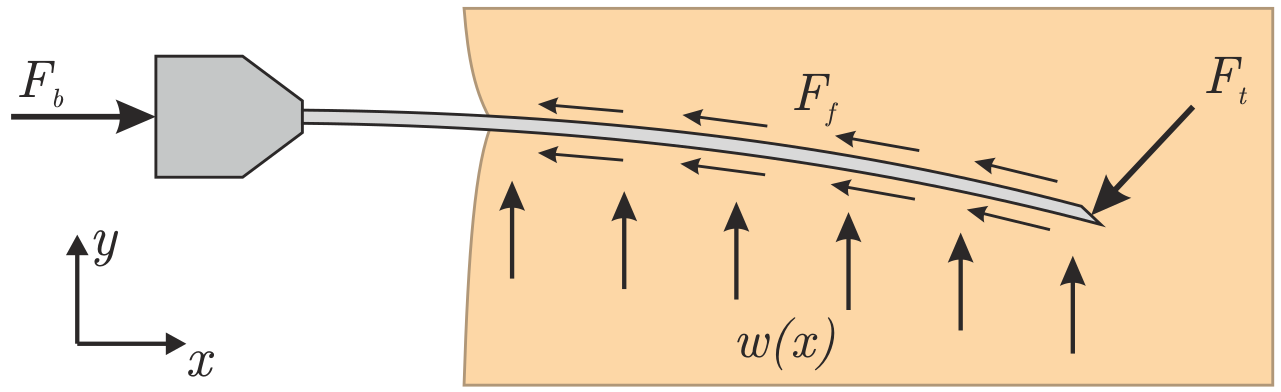
\includegraphics[width=1.0\textwidth]{Fig/chap2/roesthius_needle_forces.png}
\caption{Point and distributed forces acting on the needle during insertion\cite{roesthuis_mechanics-based_2012}.}
\label{fig:needle_forces}
\end{figure}

\begin{figure}[h]
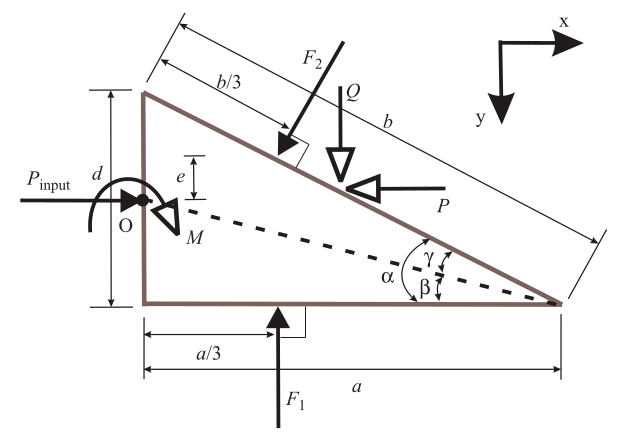
\includegraphics[width=1.0\textwidth]{Fig/chap2/misra_tip_forces.png}
\caption{Free-body diagram depicting forces acting on the needle tip during insertion into an elastic medium\cite{misra_mechanics_2010}.}
\label{fig:tip_forces}
\end{figure}

\section{Needle Modeling}
The goal of research in this area is to produce a model of needle behavior that very closely approximates its actual performance so that a needle trajectory can be planned and accurately under the assumption that little information about the needle tip is available during insertion. Most papers simplify the needle trajectory to a single bending direction in a 2D plane, but this is not representative of needle behavior during an insertion guided by continuous-rotation steering.

\subsection{Non-Holonomic Kinematics}
The non-holonomic kinematics of a beveled-tip needle can be represented by modeling the needle as a bicycle with the front wheel fixed at a constant steering angle\cite{webster_nonholonomic_2006,cowan_robotic_2011}. Since the steering angle is determined by the shape of the needle, the stiffness of the tissue, and the velocity of insertion, it must be calculated for each combination of variables.

\begin{figure}[h]
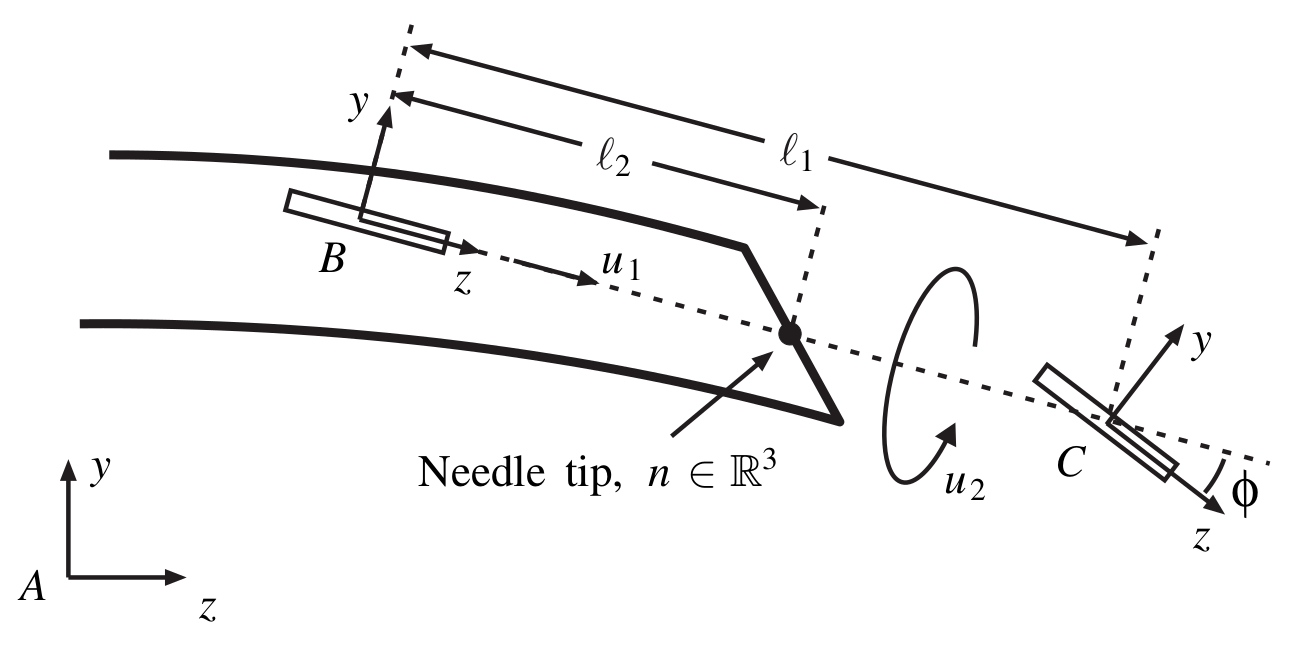
\includegraphics[width=1.0\textwidth]{Fig/chap2/webster_nonholonomic_model.png}
\caption{Nonholonomic model in which the needle tip is represented as a bicycle with a fixed front-wheel steering angle\cite{webster_nonholonomic_2006}.}
\label{fig:webster_nonholonomic_model}
\end{figure}

Subsequent work accounts for forces on the needle that cannot be modeled as components of the steering angle, such as dynamic friction and torsion in the needle shaft\cite{reed_modeling_2009, swensen_torsional_2014}.

\subsection{Finite Element Models}
Finite Element (FE) modeling of the needle and surrounding medium addresses some of the drawbacks of the kinematic needle model, such as the ability to model inconsistent deflection when inserting through nonhomogeneous tissue\cite{goksel_modeling_2009}. FEM-based approaches use several types of finite elements, including angular springs and beam elements. While the problem is often simplified as a 2D mesh in a plane, the approach is extensible to 3D\cite{chentanez_interactive_2009}.

FE modeling necessitates explicit representations for the sliding interface between the needle shaft and the surrounding tissue and for the elastic mechanical properties that govern the deformation of tissue during insertion\cite{dehghan_comparison_2006}. Since needles are very slender and the magnitude of deflection is comparatively large, the assumption of linear displacement usually used during FE analysis is not applicable and a computationally-intensive numerical solver is required to solve for nonlinear displacement.

\begin{figure}[h]

\includegraphics[width=1.0\textwidth]{Fig/placeholder.png}
\caption{Finite element model which represents the needle as a series of angular springs interacting with a 2D mesh\cite{goksel_modeling_2009}.}
\label{fig:needle_fe_model}
\end{figure}

\subsection{Mechanical Models}
Other works model the needle as an Euler-Bernoulli beam, with the forces acting on the needle divided into a force acting on the needle tip and a distributed load acting on the needle shaft. The tip force is related to the force required to cut through the tissue, which depends on the insertion velocity\cite{barnett_fracture_2015}. The distributed shaft load is related to the stiffness and viscous coefficient of the tissue\cite{abayazid_integrating_2013}.

Another approach is to represent the shape of the needle as a polynomial and use mechanical bending energy to choose the polynomial coefficients\cite{roesthuis_modeling_2015,misra_mechanics_2010,abayazid_integrating_2013}. This accounts for needle deflection and deformation of surrounding tissue, which allows calculation of the force on the needle base.

Mechanical models require direct measurement of the elastic modulus, stiffness, and cutting force of the tissue and the elastic modulus of the needle. The tissue is generally assumed to be homogeneous for simplicity.

\begin{figure}[h]

\includegraphics[width=1.0\textwidth]{Fig/placeholder.png}
\caption{Mechanical model of a needle in a two-bend configuration\cite{roesthuis_mechanics-based_2012}.}
\label{fig:needle_mech_model}
\end{figure}


\section{Needle Steering}

The different approaches to needle steering can be generalized as minimally-invasive methods to guide a needle to a desired point in the body using control inputs applied outside the body. The various methods produced in this line of research can be placed along a spectrum of mechanical complexity at the needle tip, ranging from methods for steering a needle using only control inputs at its base, to needles with some actuation at the tip and along the shaft, to continuum robots. 

Needle steering strategies rely on the asymmetric force at the tip of a beveled needle as a control input to direct the needle along a desired trajectory. Rotating the needle tip changes the direction of the force vector, allowing the direction of deflection to be controlled. Steering algorithms that take advantage of this behavior include duty cycle steering, CURV steering, and continuous-rotation steering.

Symmetric-tip needles are not subject to significant asymmetric tip for during insertion\cite{dimaio_needle_2003}. While the magnitude of deflection during insertion is reduced, the direction of deflection is inconsistent, so symmetric-tipped needles cannot be steered by rotating the needle tip. An alternative strategy steers the needle by moving its base outside the tissue, which induces a bend in the needle shaft\cite{glozman_image-guided_2007}.

Curved- or kinked-tip needles use similar mechanical principles to steer as beveled-tip needles, but the addition of a pre-bent section greatly increases the asymmetric force applied to the needle tip during insertion\cite{reed_integrated_2008}. This allows the needle to achieve a tighter turning radius, especially if the needle shaft is made of nitinol wire. Kinked-tip needles cause more tissue damage than beveled-tip needles when steered using a rotation-based strategy, but needles with passively-actuated tips have been developed to mitigate this by straightening during continuous rotation\cite{swaney_flexure-based_2013}. Needles with fully-actuated tips can be steered along a trajectory without rotating the needle\cite{roesthuis_modeling_2015}. A disadvantage of curved-tip needles is that the tip translates during rotation, which violates the assumption of the nonholonomic kinematic model that the needle will only move along the tip vector\cite{reed_integrated_2008}.

\begin{figure}[h]

\includegraphics[width=1.0\textwidth]{Fig/placeholder.png}
\caption{Example of a needle with a pre-curved tip\cite{reed_integrated_2008}.}
\label{fig:kinked_tip}
\end{figure}

\begin{figure}[h]
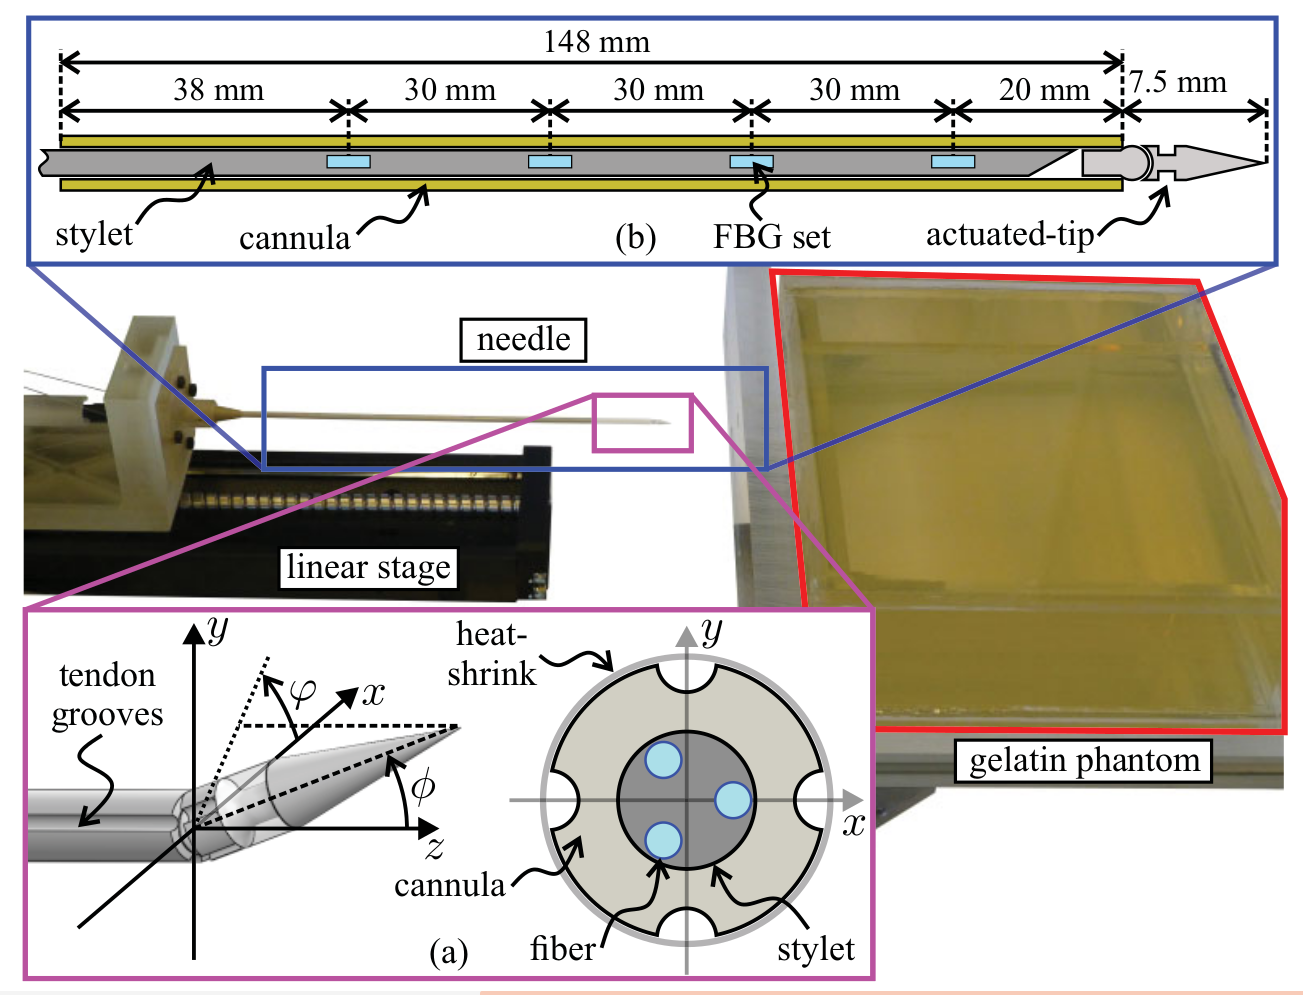
\includegraphics[width=1.0\textwidth]{Fig/chap2/actuated_tip_needle.png}
\caption{Custom-manufactured steerable needle with an actuated tip and Fiber Bragg Grating strain gauges\cite{roesthuis_modeling_2015}.}
\label{fig:actuated_tip}
\end{figure}

Concentric-tube needles consist of several nested pre-bent tubes\cite{webster_mechanics_2009, rucker_geometrically_2010, dupont_design_2010-1}. The needle can be actively curved or straightened by rotating the tubes so their directions of curvature are aligned or in opposition. These needles experience potentially-undesired releases of energy when the concentric elements snap between equilibrium states.

- Problems with these approaches, and with approaches that use custom needles in general, is that there aren't any clinically-available biopsy needles of these types. Need to be able to steer straight beveled-tip needles if we want to use what's out there right now.

- Potential for tissue damage along insertion trajectory is risky.

\begin{figure}[h]
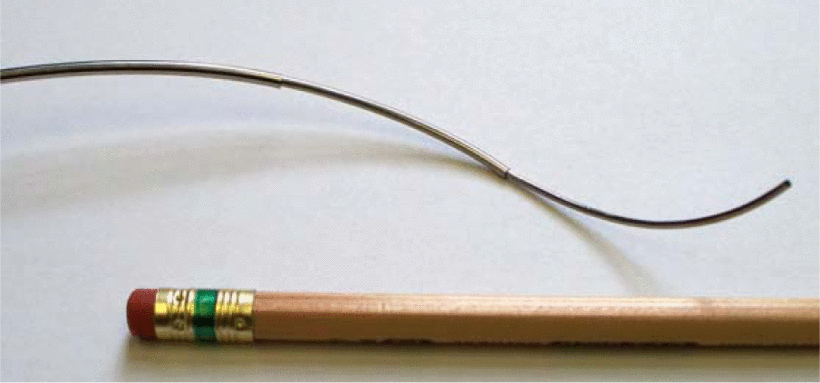
\includegraphics[width=1.0\textwidth]{Fig/chap2/concentric_needle.png}
\caption{Example of a steerable concentric-tube needle\cite{rucker_geometrically_2010}.}
\label{fig:concentric_tubes}
\end{figure}


- TODO: (Fichera) Add more different types of needles. Add figures of needle tips to support and keep the reader (i.e. Loris) engaged.

- TODO: (Fichera) Support the claim that stiff biopsy needles are the current clinical standard.




\section{Needle Localization}
Existing work in needle localization generally operates on individual scans or video frames in isolation. It would be very useful to use the results from processing a previous image to find the needle in the current image. Adding the change in the forward kinematics of the needle would improve this processing as well.

\subsection{Coronal and Sagittal Plane Imaging}
Prior work by our research group demonstrated closed-loop MR imaging in the coronal and sagittal planes to follow the needle during insertion\cite{patel_closed-loop_2015}. The needle tip is captured in each scan and its measured position of the centroid of the tip artifact is used to plan the pose of the subsequent scan in the perpendicular plane. The field of view of each plane is sized based on the maximum anticipated deflection of the needle between scans.

\begin{figure}[h]
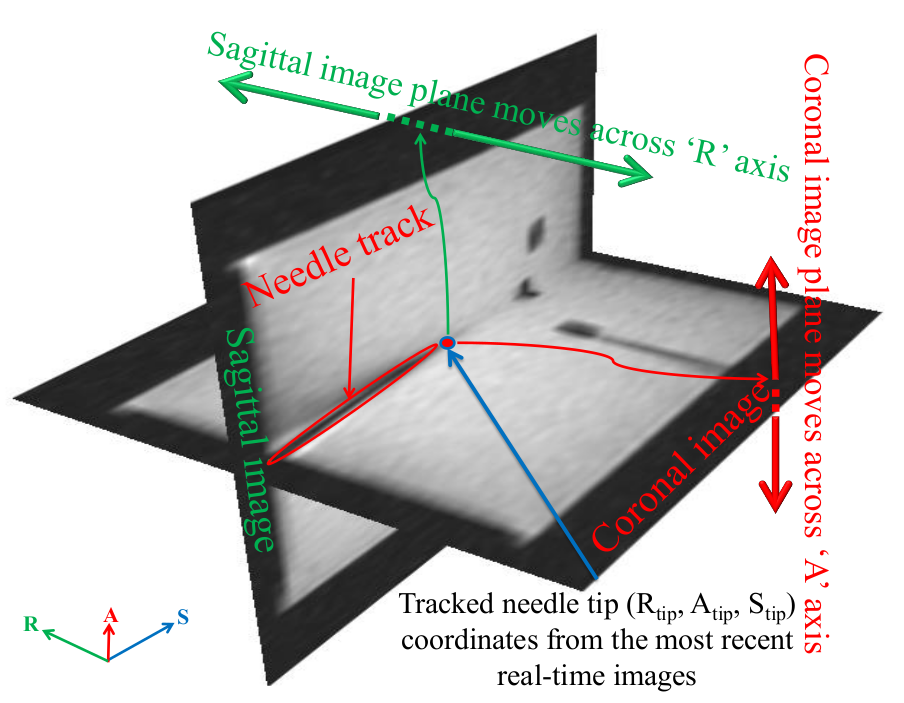
\includegraphics[width=1.0\textwidth]{Fig/chap2/patel_mri_tracking.png}
\caption{Alternating-planes strategy to track the needle tip during insertion\cite{patel_closed-loop_2015}.}
\label{fig:needle_guide}
\end{figure}

A risk with imaging in a plane parallel to the needle shaft is potential loss of tracking if the needle tip is not found in one of the scans. This risk can be mitigated by choosing a thick scan plane sized to capture the worst-case needle deflection between scans. High scan plane thickness reduces the clarity of features in MR images, which would be detrimental for identifying anatomical features near the needle.


\subsection{Transverse Plane Imaging}
Imaging in the plane normal to the needle shaft captures the needle in cross-section. This avoids the problem of imaging in a plane that does not contain the needle, but it is more challenging to find the plane containing the needle tip. For US scanning the transducer can be mounted on a motorized platform and moved in synchronization with the needle base to capture the same point on the needle in cross-section throughout insertion\cite{carriere_needle_2015,rossa_adaptive_2016}.

\begin{figure}[h]
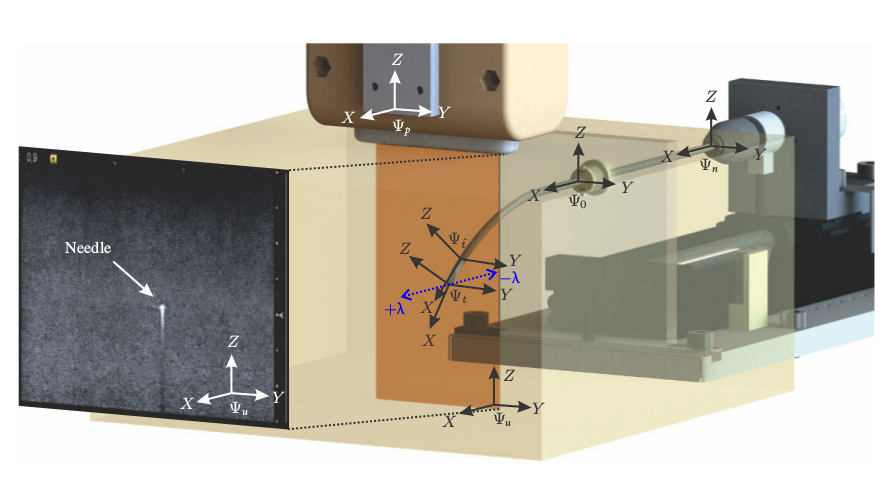
\includegraphics[width=1.0\textwidth]{Fig/chap2/vrooijink_US_tracking.png}
\caption{Needle tracking in US via imaging in the transverse plane\cite{vrooijink_needle_2014}.}
\label{fig:transverse_planes_us}
\end{figure}

\subsection{3D Imaging}
NeedleFinder is a 3D Slicer extension for needle localization and segmentation\cite{pernelle_validation_2013}. Given a manually-selected tip position, NeedleFinder searches through sequential axial scan planes and finds the cross-sections of the voids created by needle and catheter artifacts in each layer. An angular-spring finite element model defined by the shape and stiffness of the needle is fit to the detected needle points. Manual selection of the needle tips is required because of the difficulty of automatically distinguishing the needles from anatomical features and noise in the MR images.

\begin{figure}[h]
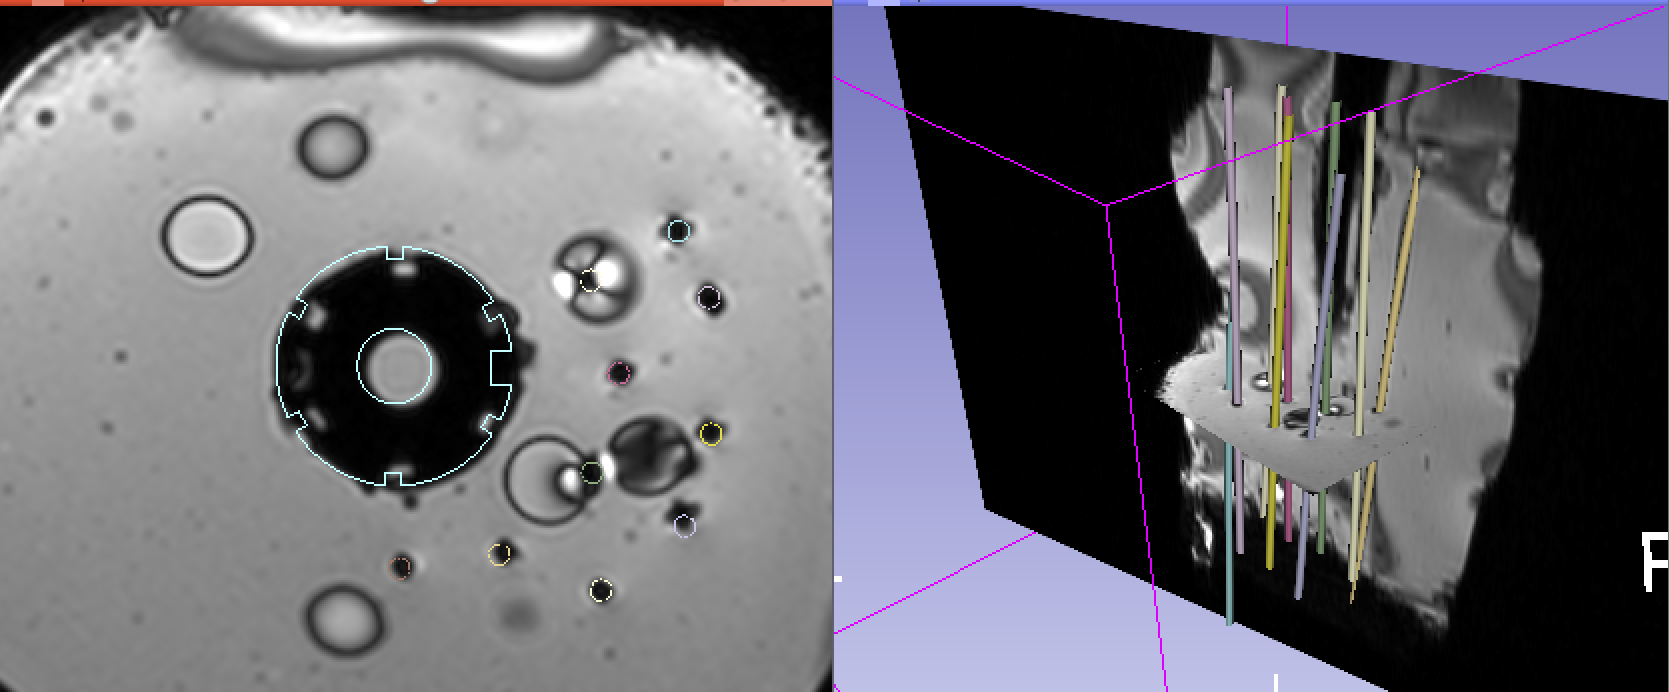
\includegraphics[width=1.0\textwidth]{Fig/chap2/needlefinder.png}
\caption{Catheters semi-automatically segmented in 3D MRI data using the NeedleFinder Slicer extension\cite{pernelle_validation_2013}.}
\label{fig:needlefinder}
\end{figure}

Other research models susceptibility artifact shapes for metal fiducial markers in MR data to automatically segment the markers and determine their poses\cite{zijlstra_fast_2017}. This approach could probably be extended to detect needle tip poses from tip artifacts with greater precision than thresholding by intensity, but the variation in the needle artifact with the orientation of the needle relative to the direction of the magnetic field would present some challenges.

In both US and MR images, the time required to resolve a 3D volume is higher than for a 2D plane, so 3D imaging is generally not suitable for real-time tracking or control.

\subsection{Non-Imaging Techniques}
An alternative method for detecting the position and shape of the needle is to add sensors to the needle to directly measure its deflection. One approach is to embed Fiber Bragg Grating optical sensors into the shaft of the needle\cite{roesthuis_three-dimensional_2014}. These sensors measure the strain in the needle as it bends and allow the shape of the needle to be calculated throughout insertion to achieve robotic steering. This approach requires specially-modified needles, precluding the use of common clinical-style biopsy needles.

\begin{figure}[h]
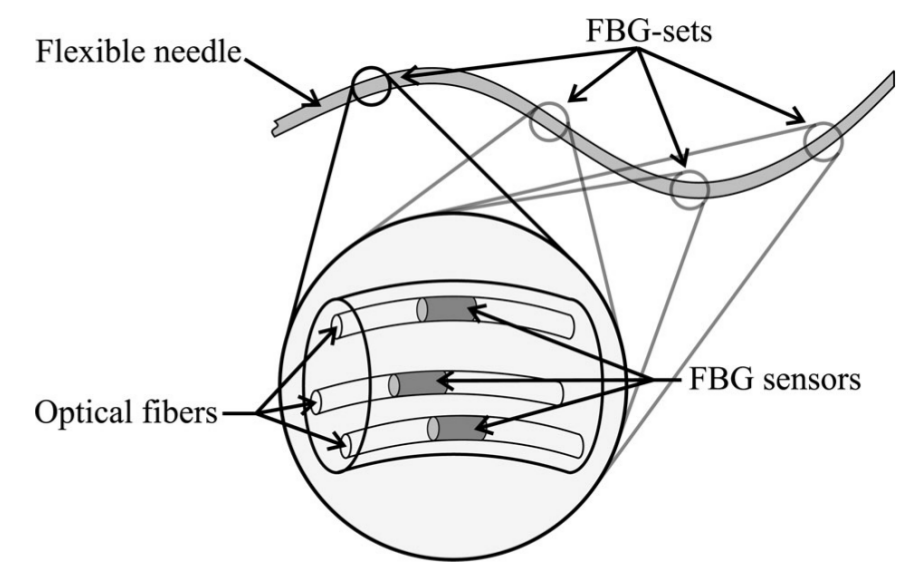
\includegraphics[width=1.0\textwidth]{Fig/chap2/fbg_needle.png}
\caption{Placement of Fiber Bragg Grating sensors on a specially-modified needle\cite{roesthuis_three-dimensional_2014}.}
\label{fig:needle_fbg}
\end{figure}

Another option is to attach magnetic tracking coils to the needle shaft and use an external sensor unit like the Polaris to measure their 6-DOF poses and compute the needle shape.
\cite{patil_needle_2014,wang_real-time_2015} This isn’t compatible with the MRI environment.






% \subsection{Needle Mechanical Modeling}
% The  model proposed by \cite{WebsterModel} uses a 2D bicycle model with a constant steering angle to capture the curving trajectory caused by the asymmetric forces on the needle tip. The dynamic model used in \cite{ReedDynamics} extends the bicycle model to include needle twist caused by friction and viscous damping along the length of the needle. \cite{SwensenDynamics} builds upon this dynamic model by adding time-variant insertion depth so that the length of the needle affected by dynamic effects varies during insertion. This hybrid kinematic/dynamic model is a middle ground between the exclusively kinematic model, which can only indirectly represent important needle mechanical behavior, and a complex finite-element model, which would need to include representations of both the needle and the surrounding soft phantom medium, as well as the friction and damping at their interface.

% \subsection{Needle Localization}
% Methods to localize a needle tip using MRI differ significantly from those used for localization via ultrasound and computer vision. As described in \cite{NeedleArtifactConfirmation} and \cite{NeedleArtifactRobotic}, the metal needle is only visible in MR imagery by interpreting the artifact caused by its interaction with the magnetic field. The size and shape of this artifact is dependent on the shape and composition of the needle, the strength of the magnetic field, and the orientation of the needle relative to the field. The shape of the artifact could be predicted and applied towards more precisely locating the needle tip.

% The localization strategy used in\cite{AIMNeedleSteering} finds the centroid of the needle tip artifact in images taken from alternating perpendicular slices. This approach produces a steady-state error relative to the true tip position, but the measurement is usable for guidance during insertion.

% The shape and extent of the needle tip artifact could be simulated using a numerical model and the physical parameters of the needle shaft and tip. [CITE] is an early effort to validate tip artifact simulations for bevel-tipped needles.


% \subsection{Needle Control}
% The needle models used by \cite{SwensenDynamics} and \cite{KallumGuidance} are designed for use with a feed-forward controller which guides the needle into a specified plane. An additional controller would steer the needle towards the target within that plane. Control in three dimensions is significantly more challenging, especially if capabilities such as trajectory planning and obstacle avoidance are desired. A 3D controller free of these constraints could calculate the desired needle steering angle using the difference between the end point of a hypothetical straight-line trajectory and the position of the target.

% [TODO: Cite CURV, duty-cycle steering, arctan steering from Hamlyn paper]
\chapter{Needle Model}
\label{sec:needlemodel} % Always give a unique label

The needle model presented in this thesis is based on minimizing the bending energy in the needle, which is represented as a beam and characterized as a parametric polynomial curve. The model is initialized with the mechanical properties of the needle and updated throughout insertion with the most recent needle base pose and the latest observed points on the needle shaft. This allows estimation of the shape of the needle using only a few new images without requiring an explicit model of the forces acting on the needle.

While other approaches to needle modeling account for bending energy, generally to determine the equilibrium state between the needle and the surrounding elastically-deformed tissue\cite{roesthuis_modeling_2015, misra_mechanics_2010, abayazid_integrating_2013}, they do not use bending energy to find the shape of the needle from observations.

Mechanics-based models make restrictive assumptions about the trajectory of the needle by limiting the number bends in the needle shaft\cite{abayazid_integrating_2013}. Models that assume a single direction of insertion\cite{roesthuis_mechanics-based_2012, abayazid_integrating_2013} cannot represent the trajectories achievable with highly-flexible needles. By parameterizing the needle coordinates independently of the insertion direction or depth, the model presented here can represent needles inserted in any direction relative to the scanner coordinate frame.

Both nonholonomic kinematic models\cite{webster_nonholonomic_2006, reed_modeling_2009, swensen_torsional_2014} and mechanics-based beam bending models\cite{roesthuis_mechanics-based_2012, abayazid_integrating_2013} require extensive characterization of the properties of the needle and the tissue in order to accurately account for the tip and shaft loads placed on the needle. Tissue properties vary between tissue types and patients, and characterization of these properties to the extent required by the needle models would probably not be practically achieveable during a procedure. In contrast, the model introduced here does not require characterization of mechanical properties, since the constraints imposed on the needle by its interaction with surrounding tissue are observed through the shape of the needle during insertion.

In the context of needle localization in MRI, it would be very time-consuming to completely and precisely evaluate the state of the needle using only observations from imaging. The core idea of this model is to take a few observations in imaging and then determine the shape of the needle through optimization that meets those constraints as well as the constraints imposed by the mechanics of the needle. Provided that the observations of the needle are distributed along the entire observable portion of its length, the needle model will be representative of the actual state of the needle to a degree of accuracy useable for guiding insertion and planning future imagery.

\section{Assumptions and Definitions}
As currently formulated, this model only considers straight needles with uniform stiffness and cross-section. Actuated devices such as flexible-tip needles and continuum robots are not considered. It is also assumed that the state of the needle relative to the camera frame is observable in imaging.

The model uses the following information about the composition and state of the needle:

\begin{itemize}
\item 6-degree-of-freedom pose of the base of the needle, via the forward kinematics of the insertion robot
\item Length of the needle
\item Diameter of the needle
\item Elastic modulus of the needle
\item Multiple observed coordinates on the needle shaft from a sparse set of cross-sectional images
\end{itemize}

Definitions of the symbols used in the needle model are provided below.

\begin{tabular}{@{}ll@{}} 
\textbf{Symbol} & \textbf{Description} \\
$C$ & cumulative cost of the needle model configuration \\
$d$ & needle shaft diameter \\
$\delta$ & needle tip offset \\
$E$ & needle shaft elastic modulus \\
$\epsilon$ & needle curve RMSE threshold \\
$I$ & second area moment of inertia \\
$k$ & observation index \\
$L$ & needle length \\
$n$ & polynomial degree \\
$\rho$ & needle curvature \\
$s$ & parametric variable \\
$U_B$ & transverse beam bending energy \\
$v $ & magnitude of deflection relative to the needle neutral axis \\
$\textbf{V}$ & vector, needle coordinate \\
$\textbf{V}_{}obs$ & vector, needle coordinate observed in imaging \\
$x \in X$ & \textbf{X-component}, set of X-components of needle coordinate \\
$y \in Y$ & \textbf{Y-component}, set of Y-components of needle coordinate \\
$z \in Z$ & \textbf{Z-component}, set of Z-components of needle coordinate \\

\end{tabular}

\section{Beam Bending Energy}
The actual biopsy needle contains several components with different mechanical properties, such as an inner rod that sides within an outer shell. Since these interactions are computationally expensive to model exactly and unnecessary to account for unless a very high degree of fidelity is desired, the model presented here simplifies the needle as a solid cylindrical beam and neglects the change in cross-sectional area at the needle tip. Under these assumptions, the area moment of inertia $I$ of the needle in cross-section is constant along the entire length of the needle, so the area moment of inertial can be calculated using Equation \ref{eq:beam_inertia}. 

\begin{equation}
\label{eq:beam_inertia}
I = \frac{\pi}{64}d^4
\end{equation}

Since the needle is assumed to have a constant diameter $d$ along its entire length, it can be represented as an Euler-Bernoulli beam with constant cross-sectional area. The transverse bending energy in a straight beam with constant cross-section, shown in Equation \ref{eq:bending_energy_transverse}, is a function of the curvature in the beam integrated over its length. Equation \ref{eq:curvature} shows the calculation of curvature in an arc. If the first derivative of the needle deflection $dv/dl$ is very small, the curvature can be approximated as Equation \ref{eq:curvature_simplified}.

\begin{equation}
\label{eq:bending_energy_transverse}
U_B = \frac{EI}{2}\int_{0}^{L}\frac{1}{\rho^2}dl
\end{equation}

\begin{equation}
\label{eq:curvature}
\frac{1}{\rho} = \frac{d^2v/dl^2}{(1+(dv/dl)^2)^{3/2}}
\end{equation}

\begin{equation}
\label{eq:curvature_simplified}
 \frac{1}{\rho} \simeq \frac{d^2v}{dl^2}
\end{equation}

In a beam subject to zero load its cumulative curvature is zero, so its total bending energy is also zero. Higher curvatures correspond to sharper bends, meaning that a beam that is predominately straight with one very sharp bend will have a greater bending energy than a beam of the same length where the bend is gentle and distributed along its entire length. Beams adopt shapes that minimize their cumulative bending energy while meeting the constraints imposed by external fixtures.

\section{Parametric Polynomial Space Curves}
The needle curve is represented using an $n$-degree parametric polynomial function, shown in Equation \ref{eq:curve_vector}. In the context of representing a needle, $n$ represents the maximum number of inflection points in each axis. Under ideal conditions a needle inserted without rotation would deflect in one direction with constant curvature, and its shape could be represented using at minimum a 3rd-degree polynomial ($n=3$).

\begin{equation}
\label{eq:curve_vector}
\textbf{V}=\begin{bmatrix}x(s) \\ y(s) \\ z(s) \end{bmatrix}=\begin{bmatrix}a_n s^n + a_{n-1} s^{n-1} + \dots + a_1 s + a_0 \\ b_n s^n + b_{n-1} s^{n-1} + \dots + b_1 s + b_0 \\ c_n s^n + c_{n-1} s^{n-1} + \dots + c_1 s + c_0 \end{bmatrix} \\
 s\in (0, 1)
 \end{equation}

%\begin{equation}
%\label{eq:parametric_curve}
%\begin{cases} x(s) = a_n s^n + a_{n-1} s^{n-1} + ... + a_1 s + a_0 \\
 %y(s) = b_n s^n + b_{n-1} s^{n-1} + ... + b_1 s + b_0  \\
 %z(s) = c_n s^n + c_{n-1} s^{n-1} + ... + c_1 s + c_0 \end{cases} \\
% s\in (0, 1)
 %\end{equation}

The three spatial coordinates $x$, $y$, and $z$ are functions of a unitless parameter $s$, which ranges from 0 at the needle base to 1 at the needle tip. Given sets of $k$ needle coordinates $\textbf{V}_{obs}$, the relationship between the values of $s$ and the positions of the needle coordinates is established by the distances between the needle coordinates, calculated in Equation \ref{eq:distance}, and the proportion of each distance to the cumulative distance between all the coordinates, calculated in Equation \ref{eq:parameter}.

\begin{equation}
\label{eq:distance}
\begin{cases}
d_k = 0 &\mbox{if } k=0 \\
%d_k = \sqrt[]{(X_k - X_{k-1})^2 + (Y_k - Y_{k-1})^2 + (Z_k - Z_{k-1})^2} &\mbox{if } k>0
d_k = \lvert \textbf{V}_{obs,k} - \textbf{V}_{obs,k-1}\rvert &\mbox{if } k>0
\end{cases}
\end{equation}

\begin{equation}
\label{eq:parameter}
\begin{cases}
s_k = 0 &\mbox{if } k=0 \\
s_k = s_{k-1} + \frac{d_k}{L_needle}&\mbox{if } k>0
\end{cases}
\end{equation}

While an alternative implementation could represent the $x$- and $y$-components of the coordinate as a function of its $z$-component, representing all three coordinates as functions of an independent parameter allows the curve to represent torturous trajectories without placing restrictions on the direction of needle insertion.

The maximum number of inflection points in each axis, and consequently the maximum number of changes in needle direction that the curve can represent, is limited by the degree of the polynomial.

\section{Curve Fitting}
The purpose of curve fitting is to choose coefficients of the parametric function in Equation \ref{eq:curve_vector} given a number of observed needle cross section coordinates so that the total bending energy in the curve and the error between the curve and the needle coordinates are minimized.

Prior to optimization, initial coefficients for each curve are found by fitting a polynomial of degree $n$ to the needle coordinates using a least-squares fit. While this initial solution is not representative of the actual mechanical factors that determine the shape of the needle, it approximates the minimum bending energy curve and helps prevent the optimization for reaching a local minimum or other failure condition.

The curve is optimized to minimize bending energy using Sequential Least SQuares Programming (SLSQP), which is an iterative constrained Non-Linear Programming (NLP) search algorithm\cite{kraft_software_1988}.

\subsection{Cost Function}
The cost function subject to minimization is shown in Equation \ref{eq:cost_function}. It is a modification of Equation \ref{eq:bending_energy_transverse} where the elastic modulus and area moment of inertia are omitted, since they are constant along the length of a straight needle with uniform cross-section.

\begin{equation}
\label{eq:cost_function}
% C = \kappa \sum_{i=0}^k \epsilon_i + \frac{EI}{2}\int_{0}^{L}\frac{1}{\rho^2}dl
C = \int_{0}^{L} \frac{1}{\rho^2}dl
\end{equation}

\subsection{Constraints}
The optimization is constrained by Equation \ref{eq:base_position_constraint} such that the coordinates of the curve at $s=0$ matches the position of the base of the needle.
% \begin{equation}
% \label{eq:base_position_constraint}
% \begin{cases} X_{k=0} = a_0 \\
%  Y_{k=0} = b_0  \\
%  Z_{k=0} = c_0 \end{cases}
%  \end{equation}
 
 \begin{equation}
 \label{eq:base_position_constraint}
 \textbf{V}_{k=0}=\begin{bmatrix} a_0 \\ b_0 \\ c_0 \end{bmatrix}
 \end{equation}

The optimization is further constrained by Equation \ref{eq:length_constraint} so that the length of the curve between $s=0$ and $s=1$ is equal to the length of the needle, and by Equation \ref{eq:rsme_constraint} so that the root-mean-square error (RMSE) between the curve and the observed points is below a specified threshold $\epsilon$.

\begin{equation}
\label{eq:length_constraint}
%L = \int_0^1 \sqrt[]{\frac{dx}{ds}^2 + \frac{dy}{ds}^2 + \frac{dz}{ds}^2} d\tau
L = \int_0^1 \lvert\frac{d\textbf{V}}{ds}\rvert ds
\end{equation}

\begin{equation}
\label{eq:rsme_constraint}
\epsilon \geq \sqrt[]{\frac{\sum_{i=0}^{k}(V_i - V_{obs,i})^2}{k}}
\end{equation}

While equality constraints can also be used to guide the optimized curve to intersect all the needle coordinates, this approach risks over-constraining the curve where the degree of the polynomial is close to the number of equality constraints.

%\subsection{Assumptions}

% TODO: (Fu) "The assumption in 3.3.4 is made but the result is not given any quantitative information. For example, in your experiment setting, “deflection of the needle tip throughout insertion is be comparatively small”, how small should it be? Will this number change when different tissue/material the needle interacts with?"

%Equations \ref{eq:distance} and \ref{eq:parameter} assumes that length of the needle model curve is close to the sum of the distances between the sampled points on the needle. This is met if the deflection of the needle tip throughout insertion is be comparatively small and the number of sample points is be sufficient to characterize the shape of the needle.

\section{Software Implementation}
Algorithm \ref{alg:update_curve_fit} shows the process of calculating polynomial coefficient to minimize bending energy given a set of observed needle coordinates. Figures \ref{fig:curve_fit_pt1}, \ref{fig:curve_fit_pt2}, and \ref{fig:curve_fit_pt3} show the process of observing points near the modeled needle curve and optimizing a new curve to match them.

%\begin{figure}[h]
%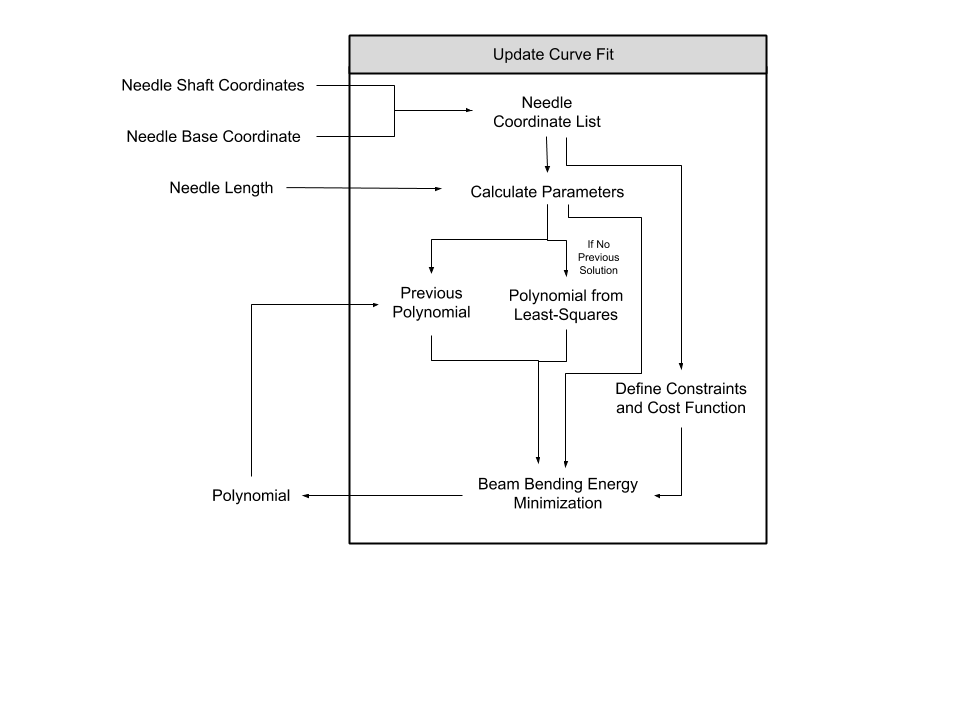
\includegraphics[width=1.0\textwidth]{Fig/chap3/Update_Curve_Fit.png}
%\caption{Flowchart for beam optimization function.}
%\label{fig:curve_fit_flow}
%\end{figure}

\begin{algorithm}
\caption{Curve Optimization}
\label{alg:update_curve_fit}
\begin{algorithmic}[1]
\Procedure{Update Curve Fit}{$coords_{needle},L_{needle},poly_{prev}$}
\State $t \gets CalculateParameters(coords_{needle}, L_{needle})$
\If {$poly_{prev} is None$}
	\State $poly_{init} \gets LeastSquares(coords_{needle})$
\Else
	\State $poly_{init} \gets poly_{prev}$
\EndIf
\State $cons \leftarrow DefineConstraints(t, coords_{needle}, L_{needle})$
\State $poly_{opt} \gets DoOptimization(poly_{init}, cons)$
\State \textbf{return} $poly_{opt}$
\EndProcedure
\end{algorithmic}
\end{algorithm}

\begin{figure}[h]
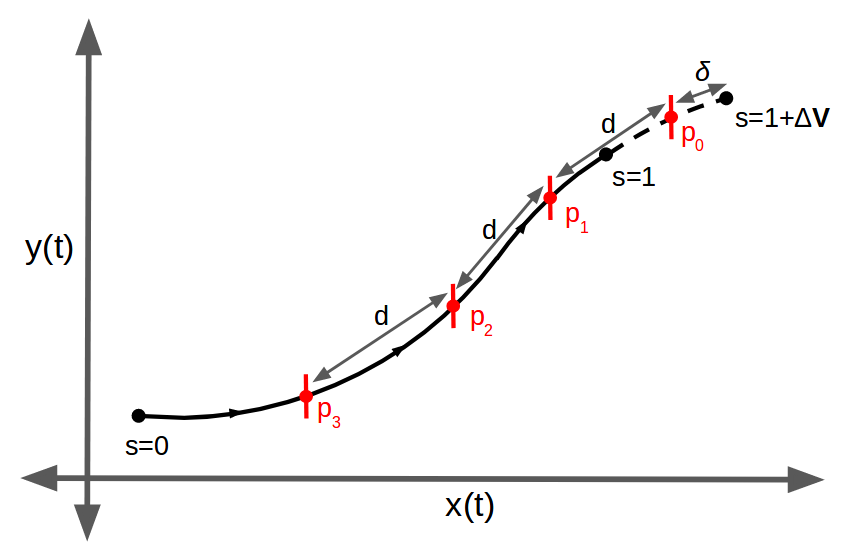
\includegraphics[width=1.0\textwidth]{Fig/chap3/curvefit_pt1.png}
\caption{Given a number of samples, the spacing between the samples $d$, the offset distance from the needle tip $\delta$, and a new needle base pose, the expected coordinate of the needle $p_k$ is calculated at each sample point.}
\label{fig:curve_fit_pt1}
\end{figure}

\begin{figure}[h]
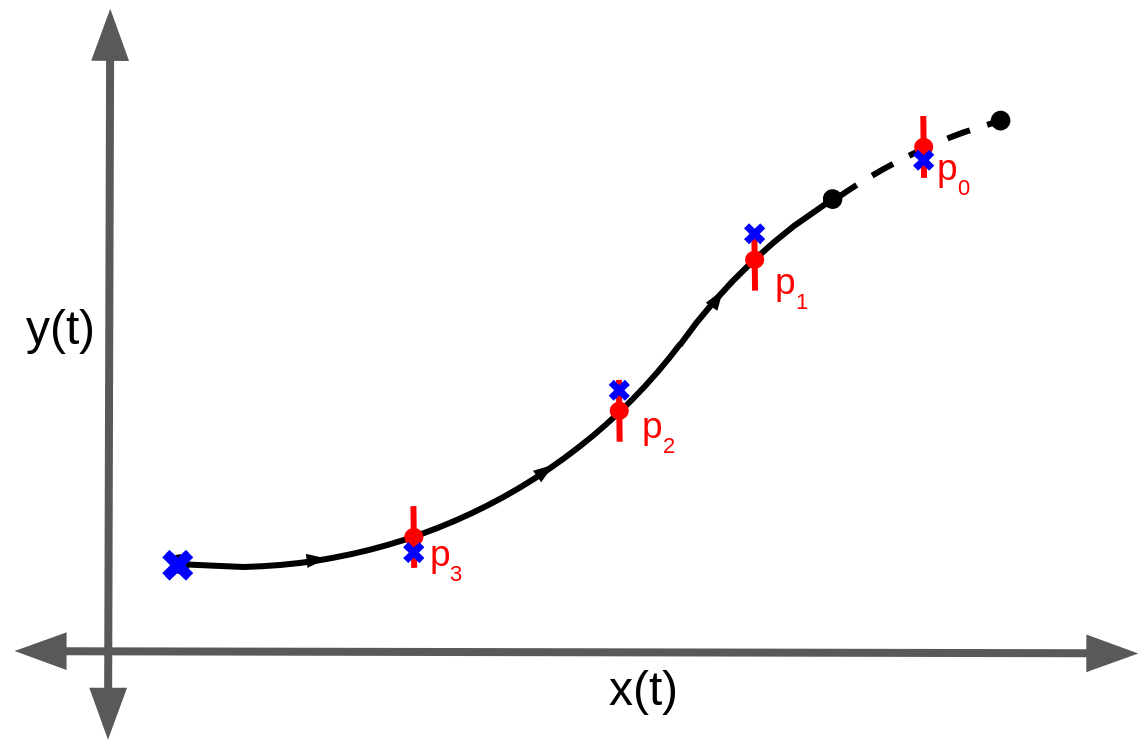
\includegraphics[width=1.0\textwidth]{Fig/chap3/curvefit_pt2.png}
\caption{New imaging is collected at each needle coordinate, and the actual position of the needle is observed.}
\label{fig:curve_fit_pt2}
\end{figure}

\begin{figure}[h]
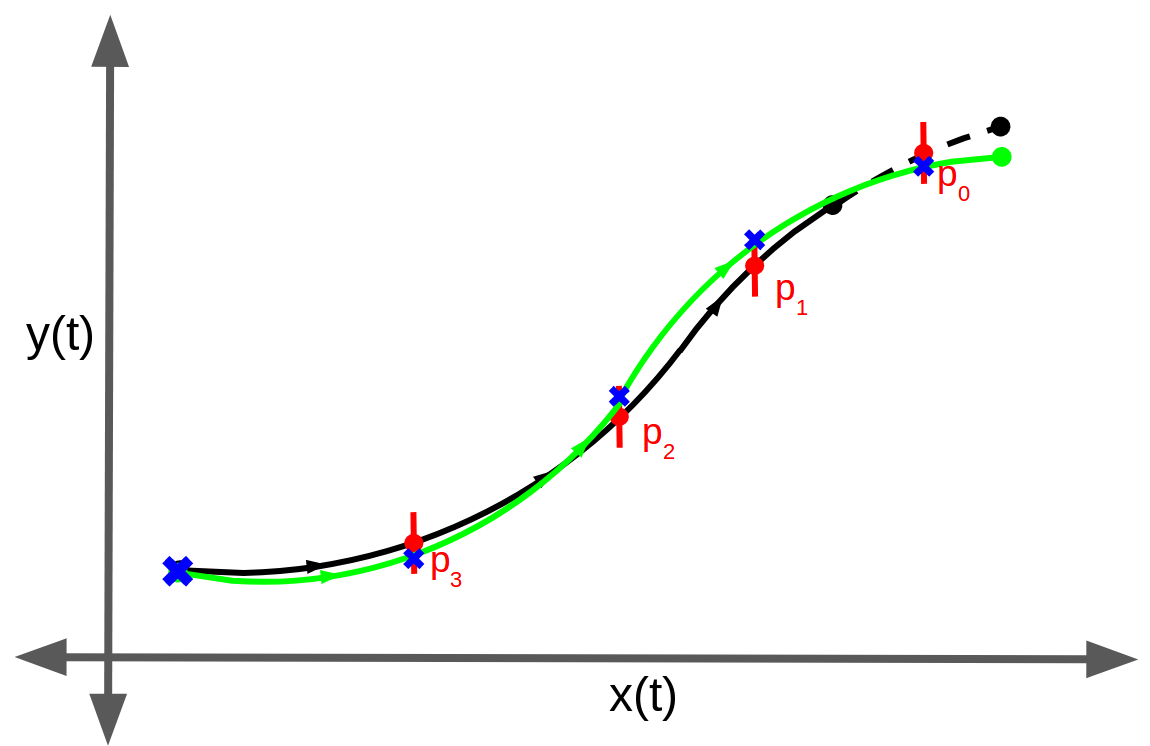
\includegraphics[width=1.0\textwidth]{Fig/chap3/curvefit_pt3.png}
\caption{A new polynomial curve is calculated, optimized to minimize both the cumulative bending energy in the needle and the error between the curve and the observed points.}
\label{fig:curve_fit_pt3}
\end{figure}


\chapter{Needle Localization in MR Images}
\label{sec:mritracking} % Always give a unique label
% use \chaptermark{}
% to alter or adjust the chapter heading in the running head

The purpose of this experiment is to validate the needle model on imagery representative of what would be available from intraoperative imagery during an MRI-guided insertion and to demonstrate a workflow suitable for real-time needle tracking.

\section{Software Architecture}
\subsection{Simulated MRI Scanner}
Full 3D MRI volumes take a long time to produce, especially if high resolution is desired: the scan time for each volume used in this thesis was approximately 5 minutes. This is a prohibitively long time in the context of real-time intraoperative imaging, so the MRI would be configured to provide 2D scans in requested planes with limited field of view. To simulate this functionality, a  Slicer module was created to resection 2D slices from each 3D volumes at specified depths.

\subsection{Needle Tracking Module}
A second Slicer module manages the needle tracking process. Figure \ref{fig:MRI_architecture} shows the architecture of this module relative to the Slicer environment and the needle modeling utility. A linear transform node is set to match the pose of the needle base in each saved volume. When commanded by the operator, the module requests slices of the MRI volume at evenly-spaced coordinates along the shaft of the needle. The thresholded image is grouped into contiguous regions, and the area and centroid are calculated for each region. The region with the centroid closest to the estimated position of the needle provided by the previous needle model curve is assumed to be the needle artifact, and the position of its centroid determines the observed position of the needle in this image. The position of the needle base is appended to this list of needle coordinates, and the combined list is used as one of the inputs for the needle curve optimization.

\begin{figure}[h]
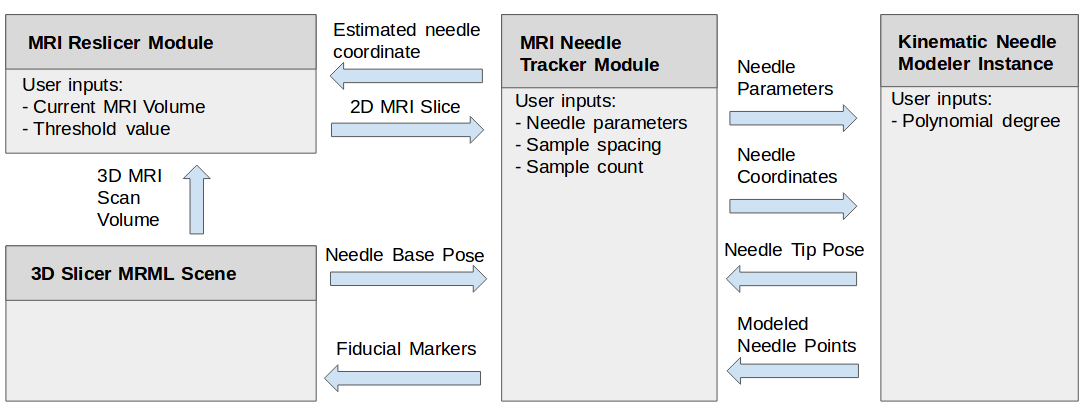
\includegraphics[width=1.0\textwidth]{Fig/chap5/MRI_software_architecture.png}
\caption{System architecture for needle detection and modeling from MRI data.}
\label{fig:MRI_architecture}
\end{figure}

\begin{figure}[h]
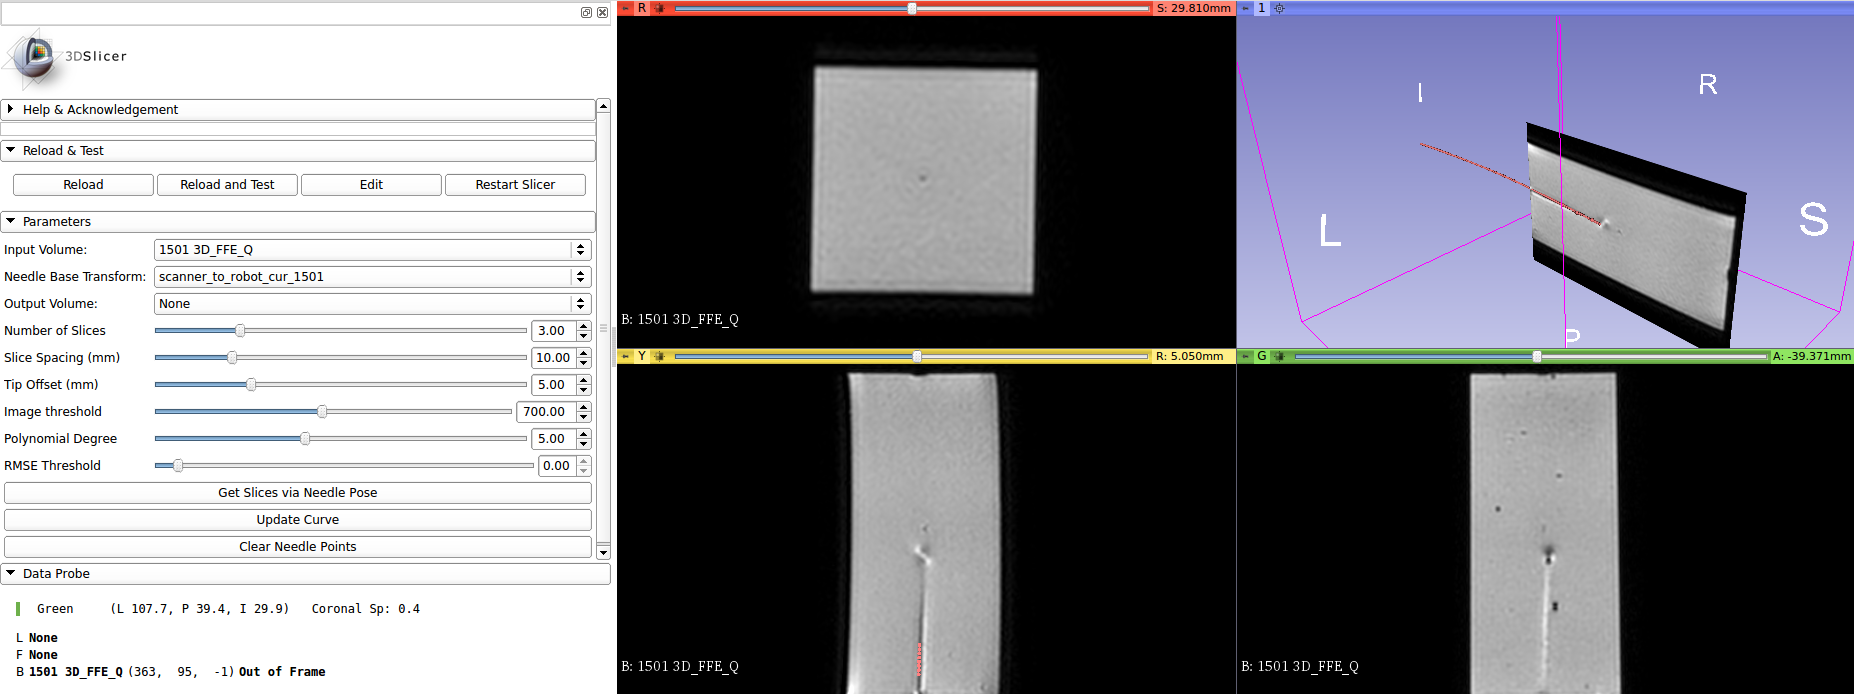
\includegraphics[width=1.0\textwidth]{Fig/chap5/MRINeedleTipTracker_module.png}
\caption{User interface for MRINeedleTipTracker 3D Slicer module.}
\label{fig:slicer_gui}
\end{figure}

\section{Experiment}

Several assumptions made to reduce the complexity of the experiment and facilitate needle tracking are listed below.

\begin{itemize}
\item A single beveled-tip clinical-style biopsy needle is to be inserted and tracked.
\item The initial vector of the needle is normal to the axial plane, and the actual pose of the needle base exactly matches the recorded pose.
\item Only homogeneous gelatin tissue phantoms are considered. The problem of identifying the needle in the presence of anatomy or other clutter is not addressed.
\item New MR data is acquired and transmitted instantaneously.
\end{itemize}

\subsection{MRI Data Collection}
The set of MRI volumes used in this experiment was captured in the 3T scanner at UMass Medical Center using a 3D Fast Field Echo protocol. The dimensions of each voxel are 0.4mm x 0.4mm x 0.5mm. The phantom used was made of agar gelatin. The needle was a 150mm stainless steel (E = 200 GPa) clinical-style biopsy needle with a beveled tip and a diameter of 2mm. Removable plastic spacers with a thickness of 5.95mm regulated the insertion distance. Two spacers were removed between scans, so the needle moves in increments of 11.9mm. Five scans were collected in total. The plastic alignment frame shown in Figure \ref{fig:needle_guide} kept the needle aligned along a known vector relative to the phantom. When used in conjunction the alignment frame and spacers allow the 6-DOF pose of the needle base to be calculated in each scan without the use of a Z-frame or external tracking equipment.

\begin{figure}[h]
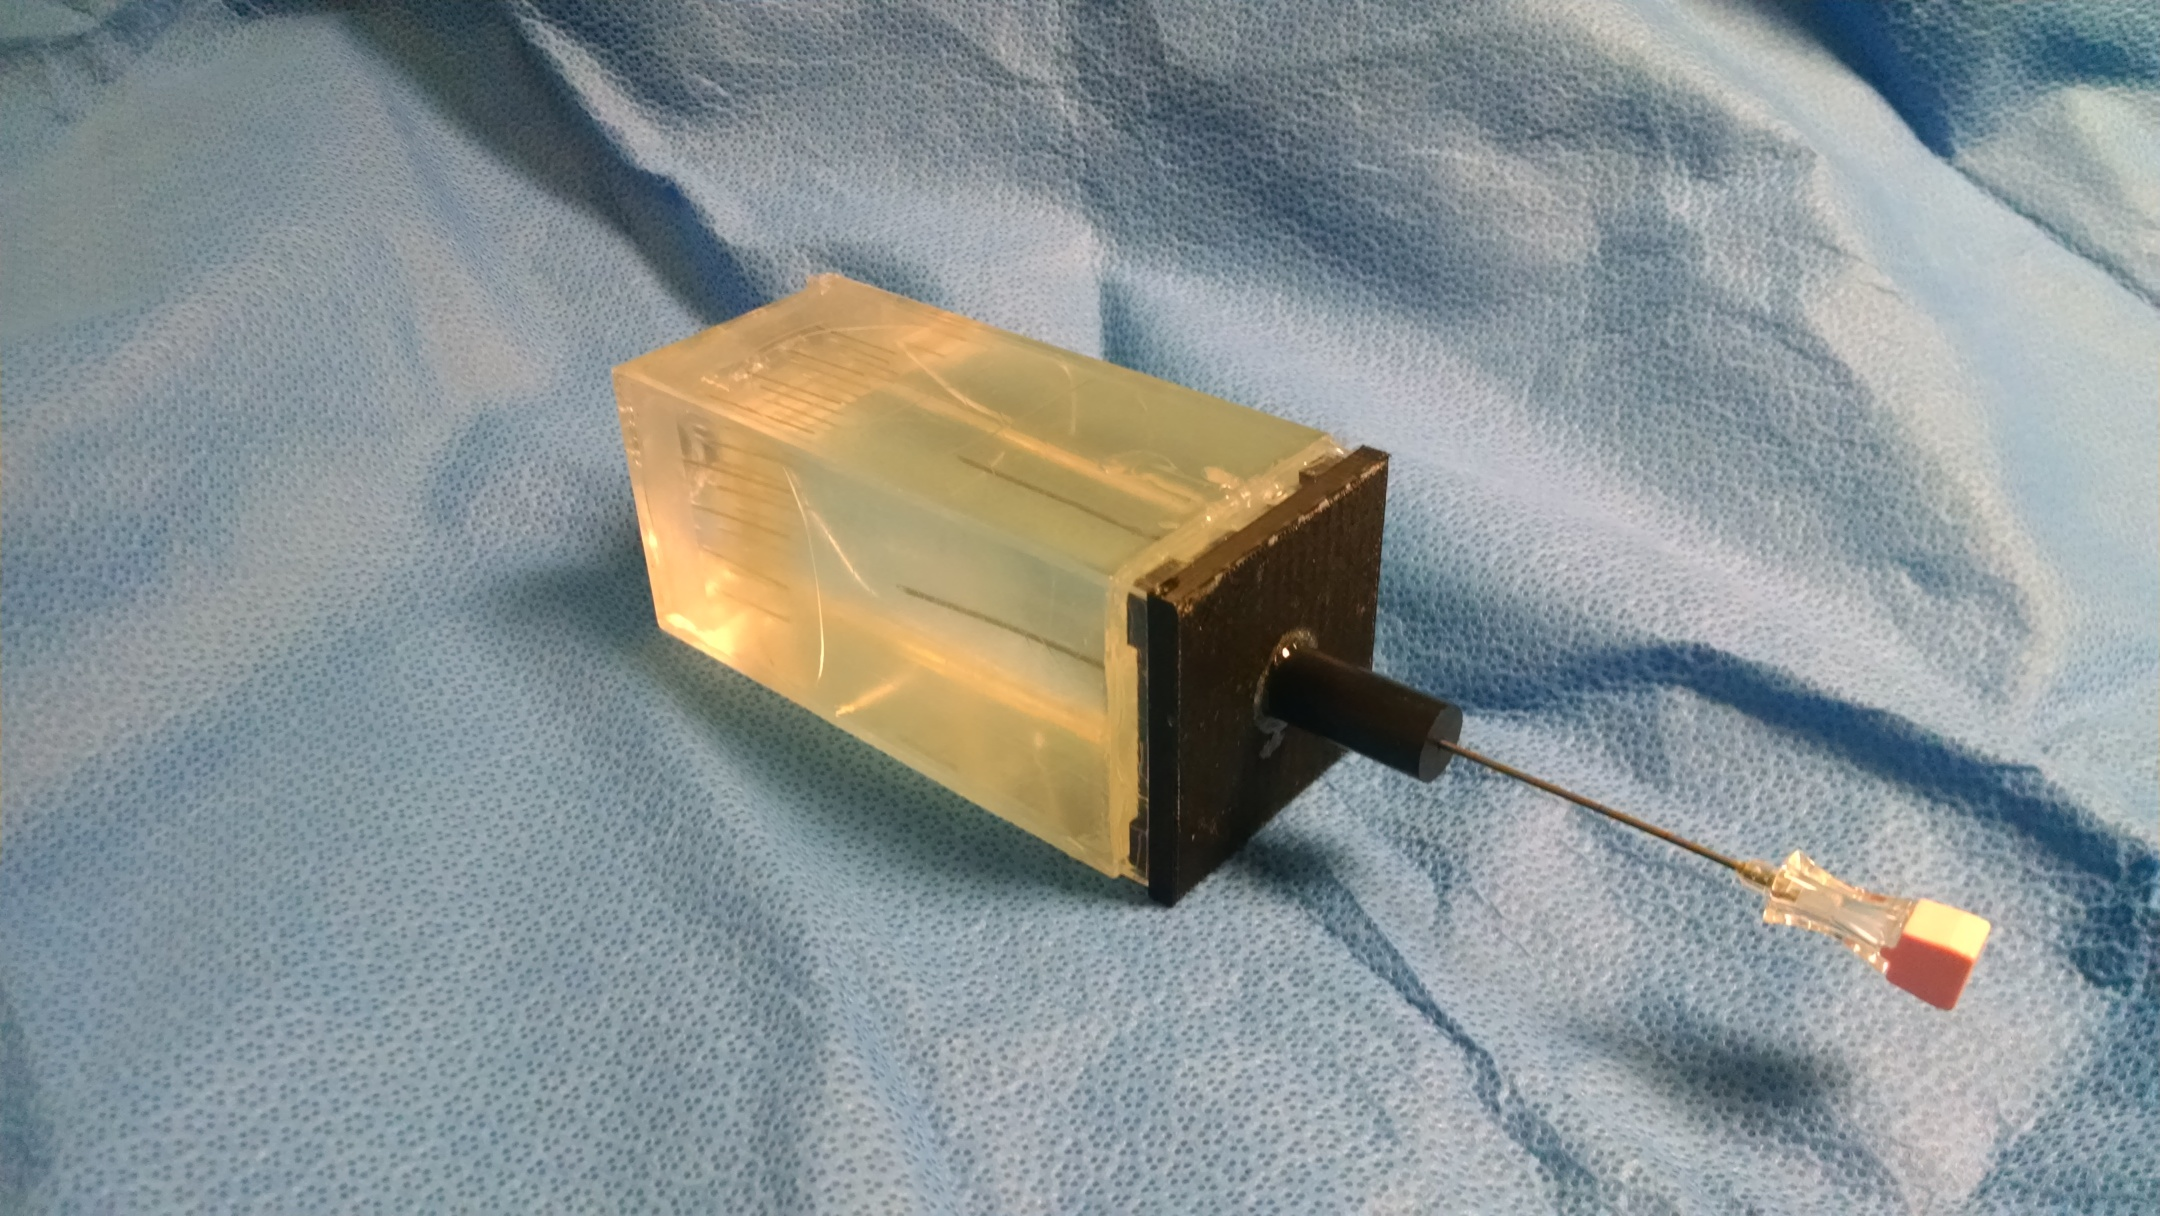
\includegraphics[width=1.0\textwidth]{Fig/chap5/phantom_with_needle_guide_small_2.jpg}
\caption{Example tissue phantom with the needle alignment frame and biopsy needle.}
\label{fig:needle_guide}
\end{figure}

\subsection{Needle Localization}

Each volume was thresholded at intensity 1500 to isolate the needle artifact. The segmentation labelmap was exported and processed separately.

The MRI volumes for each insertion step were loaded in sequence and a linear transform was set to match the pose of the needle base at each step. The needle localization algorithm was run on each dataset in turn to generate an array of points representing the simulated needle.

\section{Results}

% TODO: (Fu) "The model characterizes well the behavior of the needle with relatively small insertion distance (in Fig. 4.5, 4.6) and has a large error for large insertion depth, no matter the order of polynomial chosen, as noted in the discussion section. Is there any thought on how to improve the performance? If so, please include them in the discussion."

% TODO: (Fu) "Is it possible to compare the result with a dynamic model of the needle and vision-based state estimation?"

The baseline for the position of the needle shaft in the phantom was established by segmenting the needle artifact by intensity and computing the centroid of its cross section in every axial scan slice. Figure \ref{fig:seg_2001} shows the segmentation for the final step of the insertion, and Figure \ref{fig:ground_truth_2001} shows the positions of the centroids in successive axial planes. The error for each model is computed as the difference between the centroid coordinate and the modeled coordinate in each slice.

\begin{figure}[h]
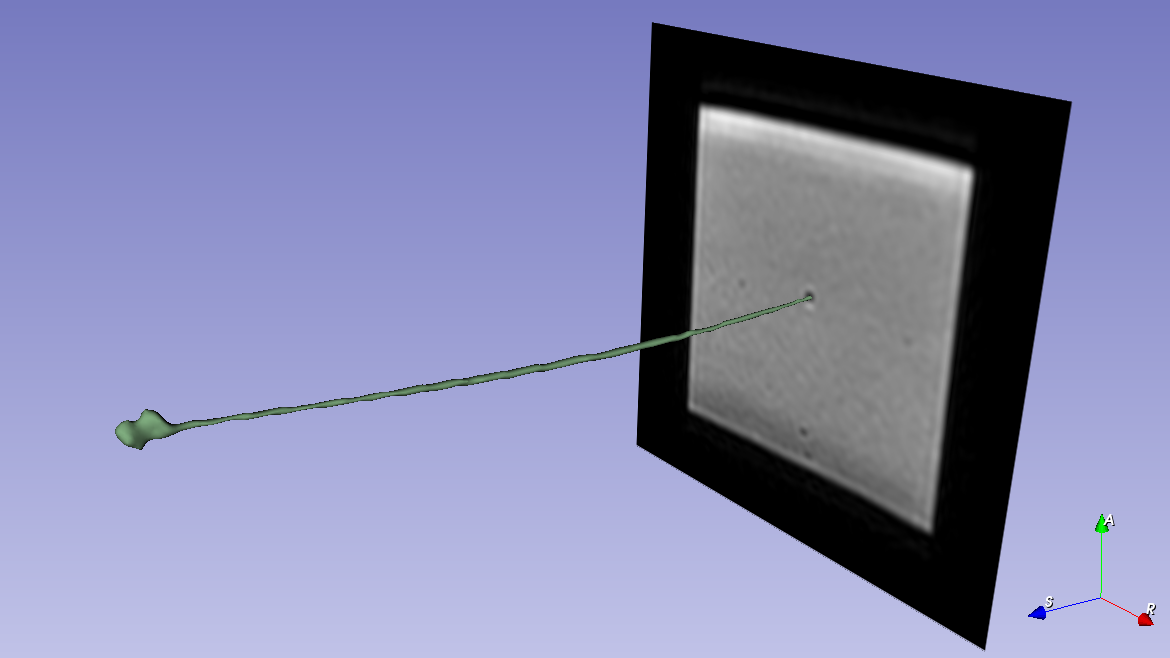
\includegraphics[width=1.0\textwidth]{Fig/chap5/segmented_artifact_2001.png}
\caption{Segmentation of needle artifact generated by thresholding MRI volume.}
\label{fig:seg_2001}
\end{figure}

\begin{figure}[h]
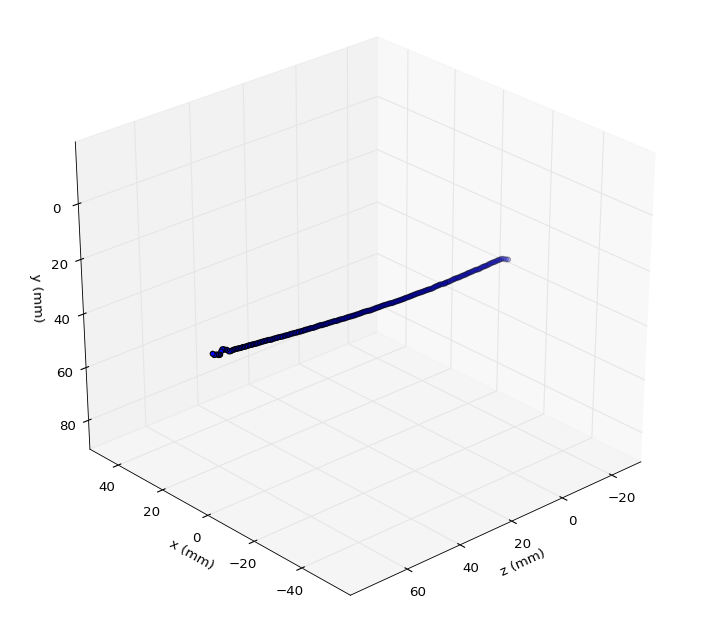
\includegraphics[width=1.0\textwidth]{Fig/chap5/neutral_axis_2001_b.png}
\caption{Baseline ground truth data, calculated from the centroids of the segmented artifact sectioned in the X-Y plane.}
\label{fig:ground_truth_2001}
\end{figure}

\subsection{Needle Localization at a Single Timestep}
\label{sec:mri_single_timestep}
At the start of curve optimization using data from a single 3D scan in isolation the needle is assumed to be a vector with magnitude matching the length of the needle. The sampling locations are placed along the needle shaft starting from the needle tip and are offset from the estimated position of the tip by a user-configurable distance to avoid sampling points within the tip artifact.

Figure \ref{fig:results_error_comparison} shows the relative error using a 1st-, 3rd-, 5th-, and 7th-degree polynomials. In this experiment the tip offset $\delta=5.0mm$, the sample spacing $d=26.0mm$, and the number of observed slices $k=3$. 

Figure \ref{fig:results_sample_comparison} shows the effect on error relative to baseline as the number of slices observed over the length of the needle is increased. 

\begin{figure}[h]
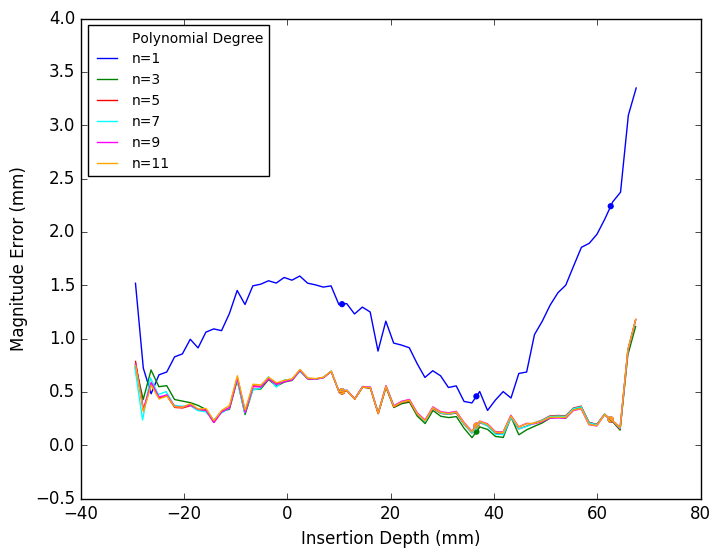
\includegraphics[width=1.0\textwidth]{Fig/chap5/errors_polynomials_3_samples.png}
\caption{Magnitude of in-plane error over insertion for various degrees of polynomial. Markers indicate the positions of the slices on the needle curve. $d=26.0mm$, $k=3$, $\delta=5.0mm$}
\label{fig:results_error_comparison}
\end{figure}

\begin{figure}[h]
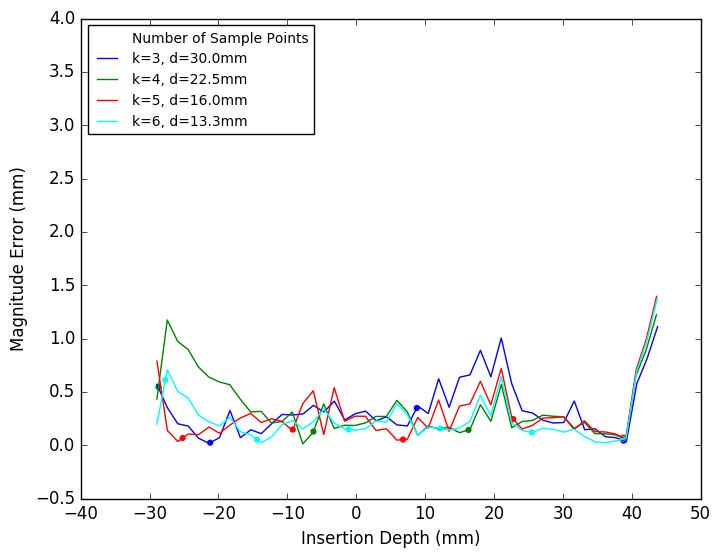
\includegraphics[width=1.0\textwidth]{Fig/chap5/errors_more_samples.png}
\caption{Magnitude of in-plane error over insertion for a variable number of sample points. Markers indicate slice positions. $n=5$, $\delta=5.0mm$}
\label{fig:results_sample_comparison}
\end{figure}

%\begin{figure}[h]
%
\includegraphics[width=1.0\textwidth]{Fig/placeholder.png}
%\caption{Example polynomial curve fit plotted against the positions of the artifact centroids in transverse plane.}
%\label{fig:curve_fit_artifact}
%\end{figure}

\subsection{Needle Localization at Sequential Timesteps}
Needle tracking in a sequence of images consists of repeated application of the method for an individual timestep described in \ref{sec:mri_single_timestep}. The optimized curve from the previous localization step is used as the initial estimate for the next localization step.

Figure \ref{fig:scan_slices} shows the positions of the scan planes and Figure \ref{fig:curve_points} shows points along the optimized curve for each insertion interval. Figure \ref{fig:curve_errors_fixed_spacing} shows the magnitude of error relative to the baseline for the optimized curve at each interval. Figure \ref{fig:curve_errors_variable_spacing} shows the magnitude of error when the spacing between the slices is increased as the needle is inserted.

\begin{figure}[h]
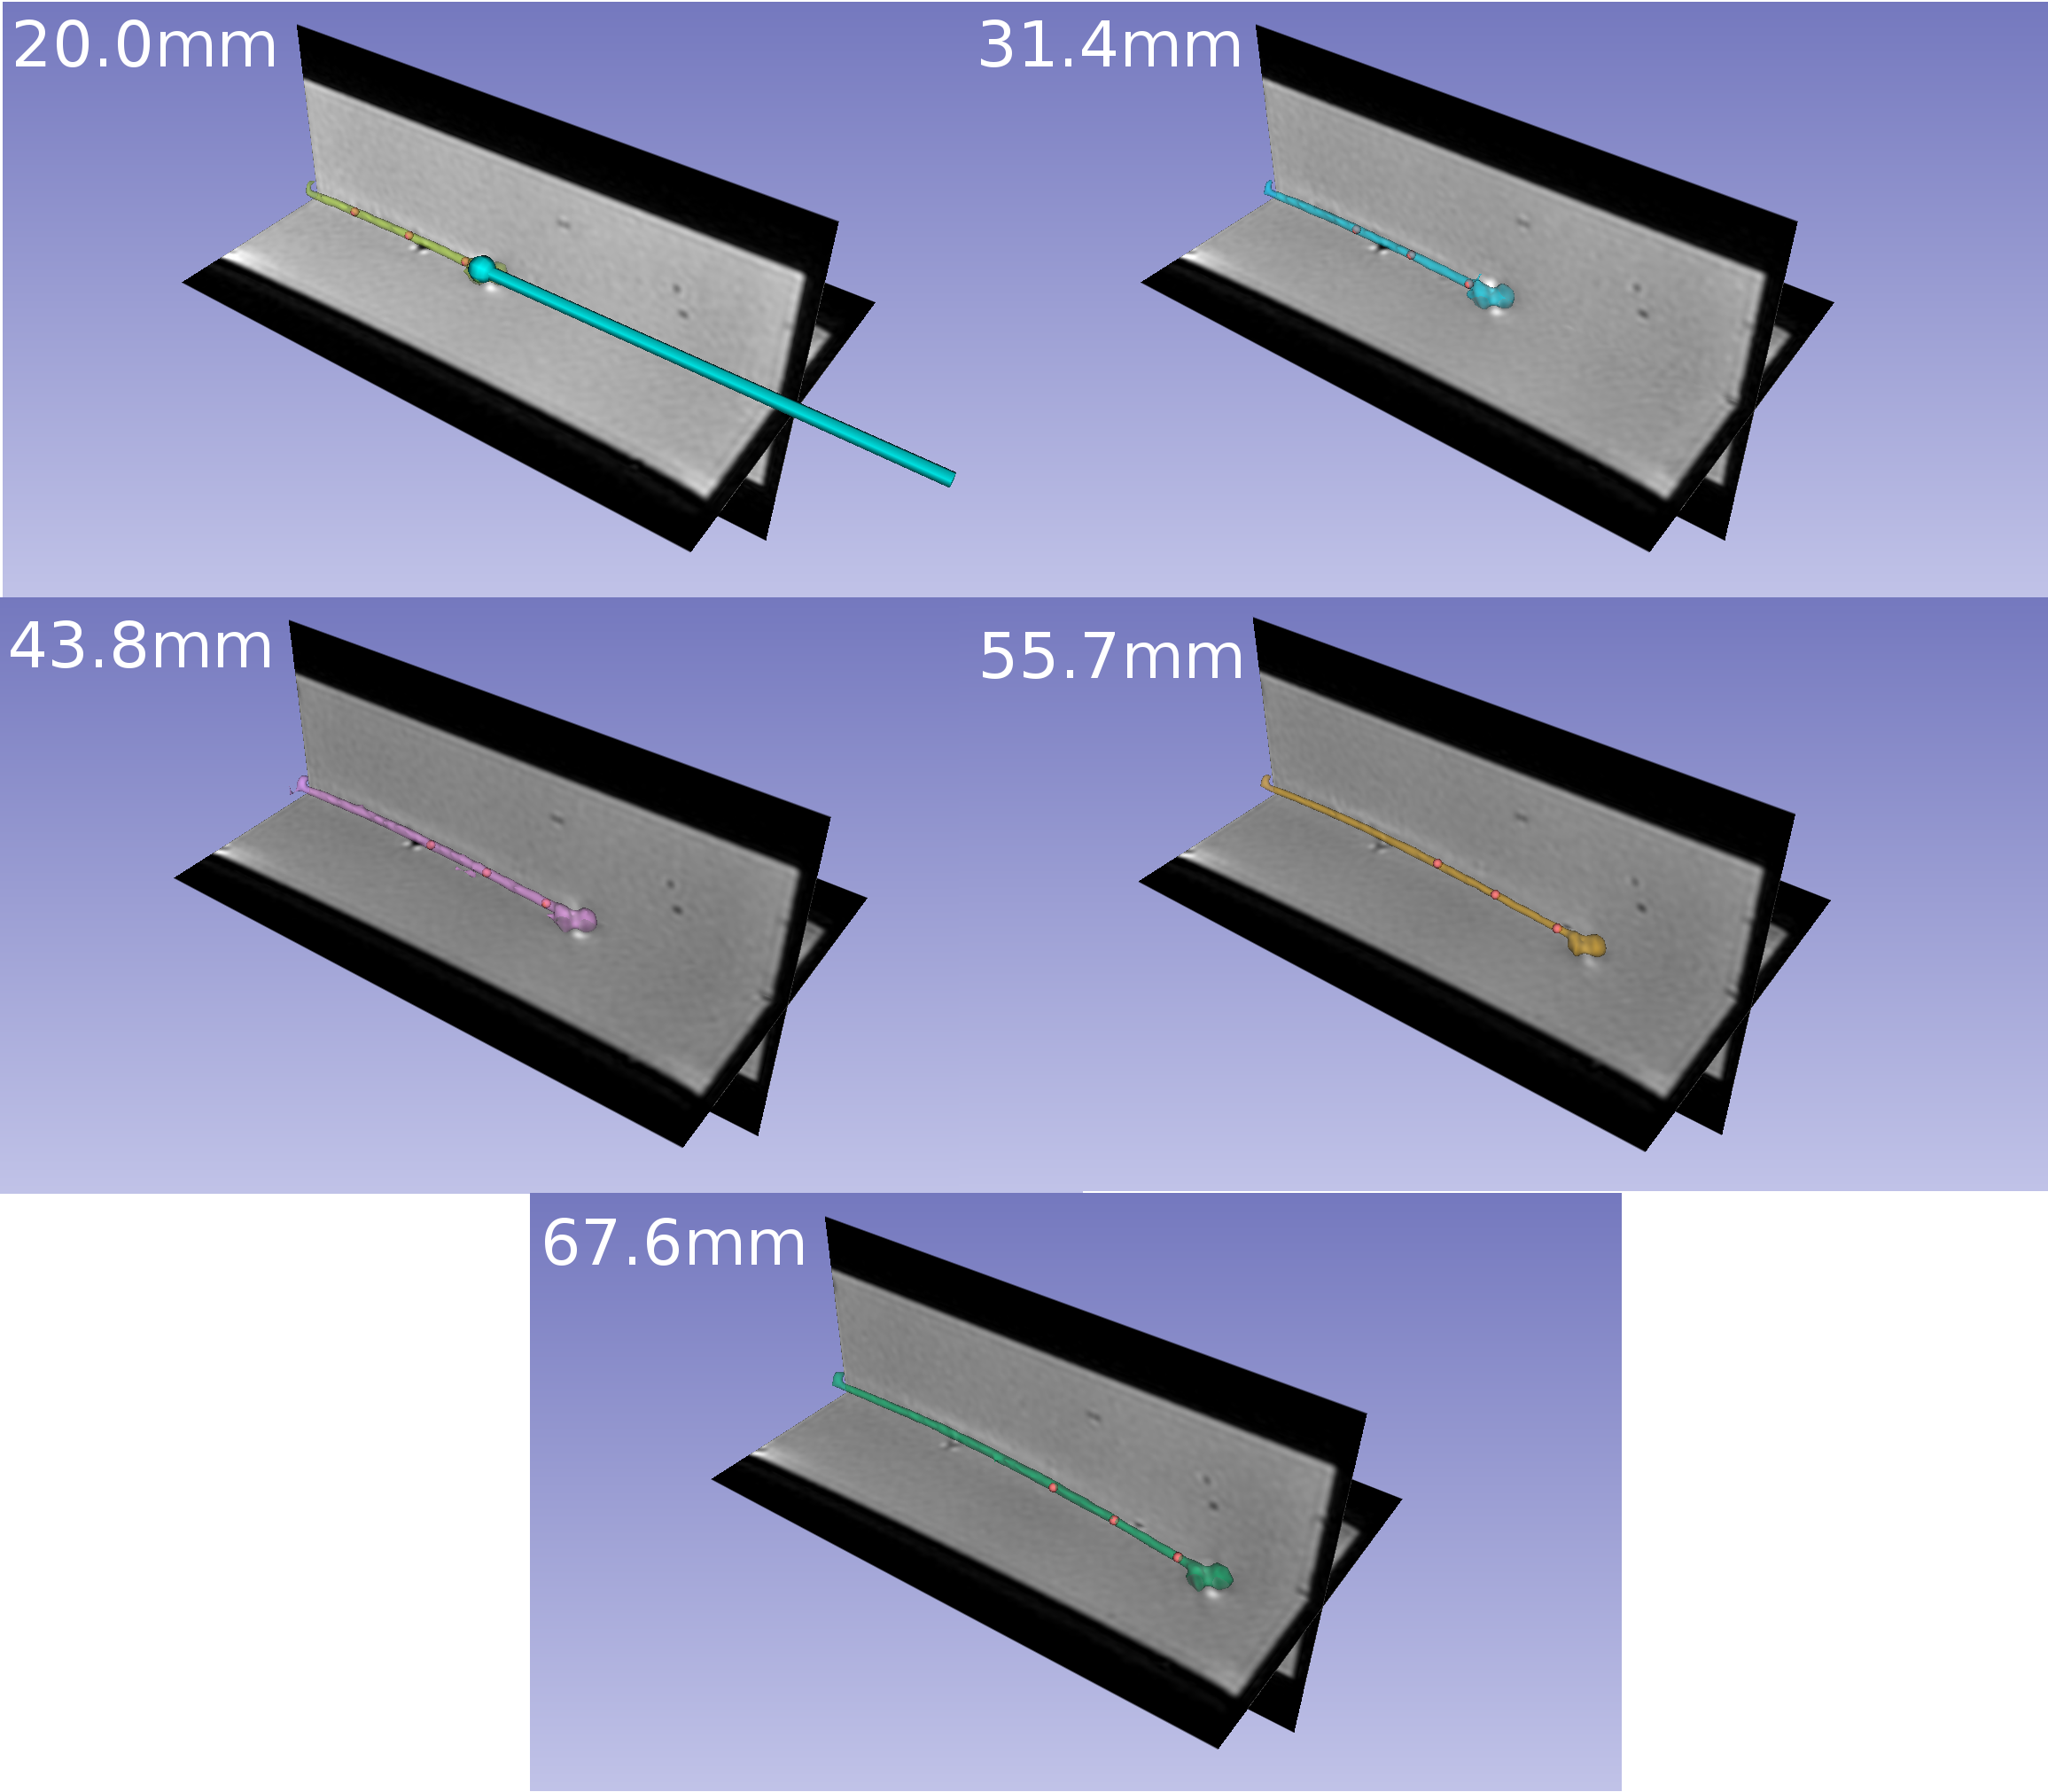
\includegraphics[width=1.0\textwidth]{Fig/chap5/scan_slices_labels.png}
\caption{Positions of 2D scan planes at each insertion step, with segmented artifact.}
\label{fig:scan_slices}
\end{figure}

\begin{figure}[h]
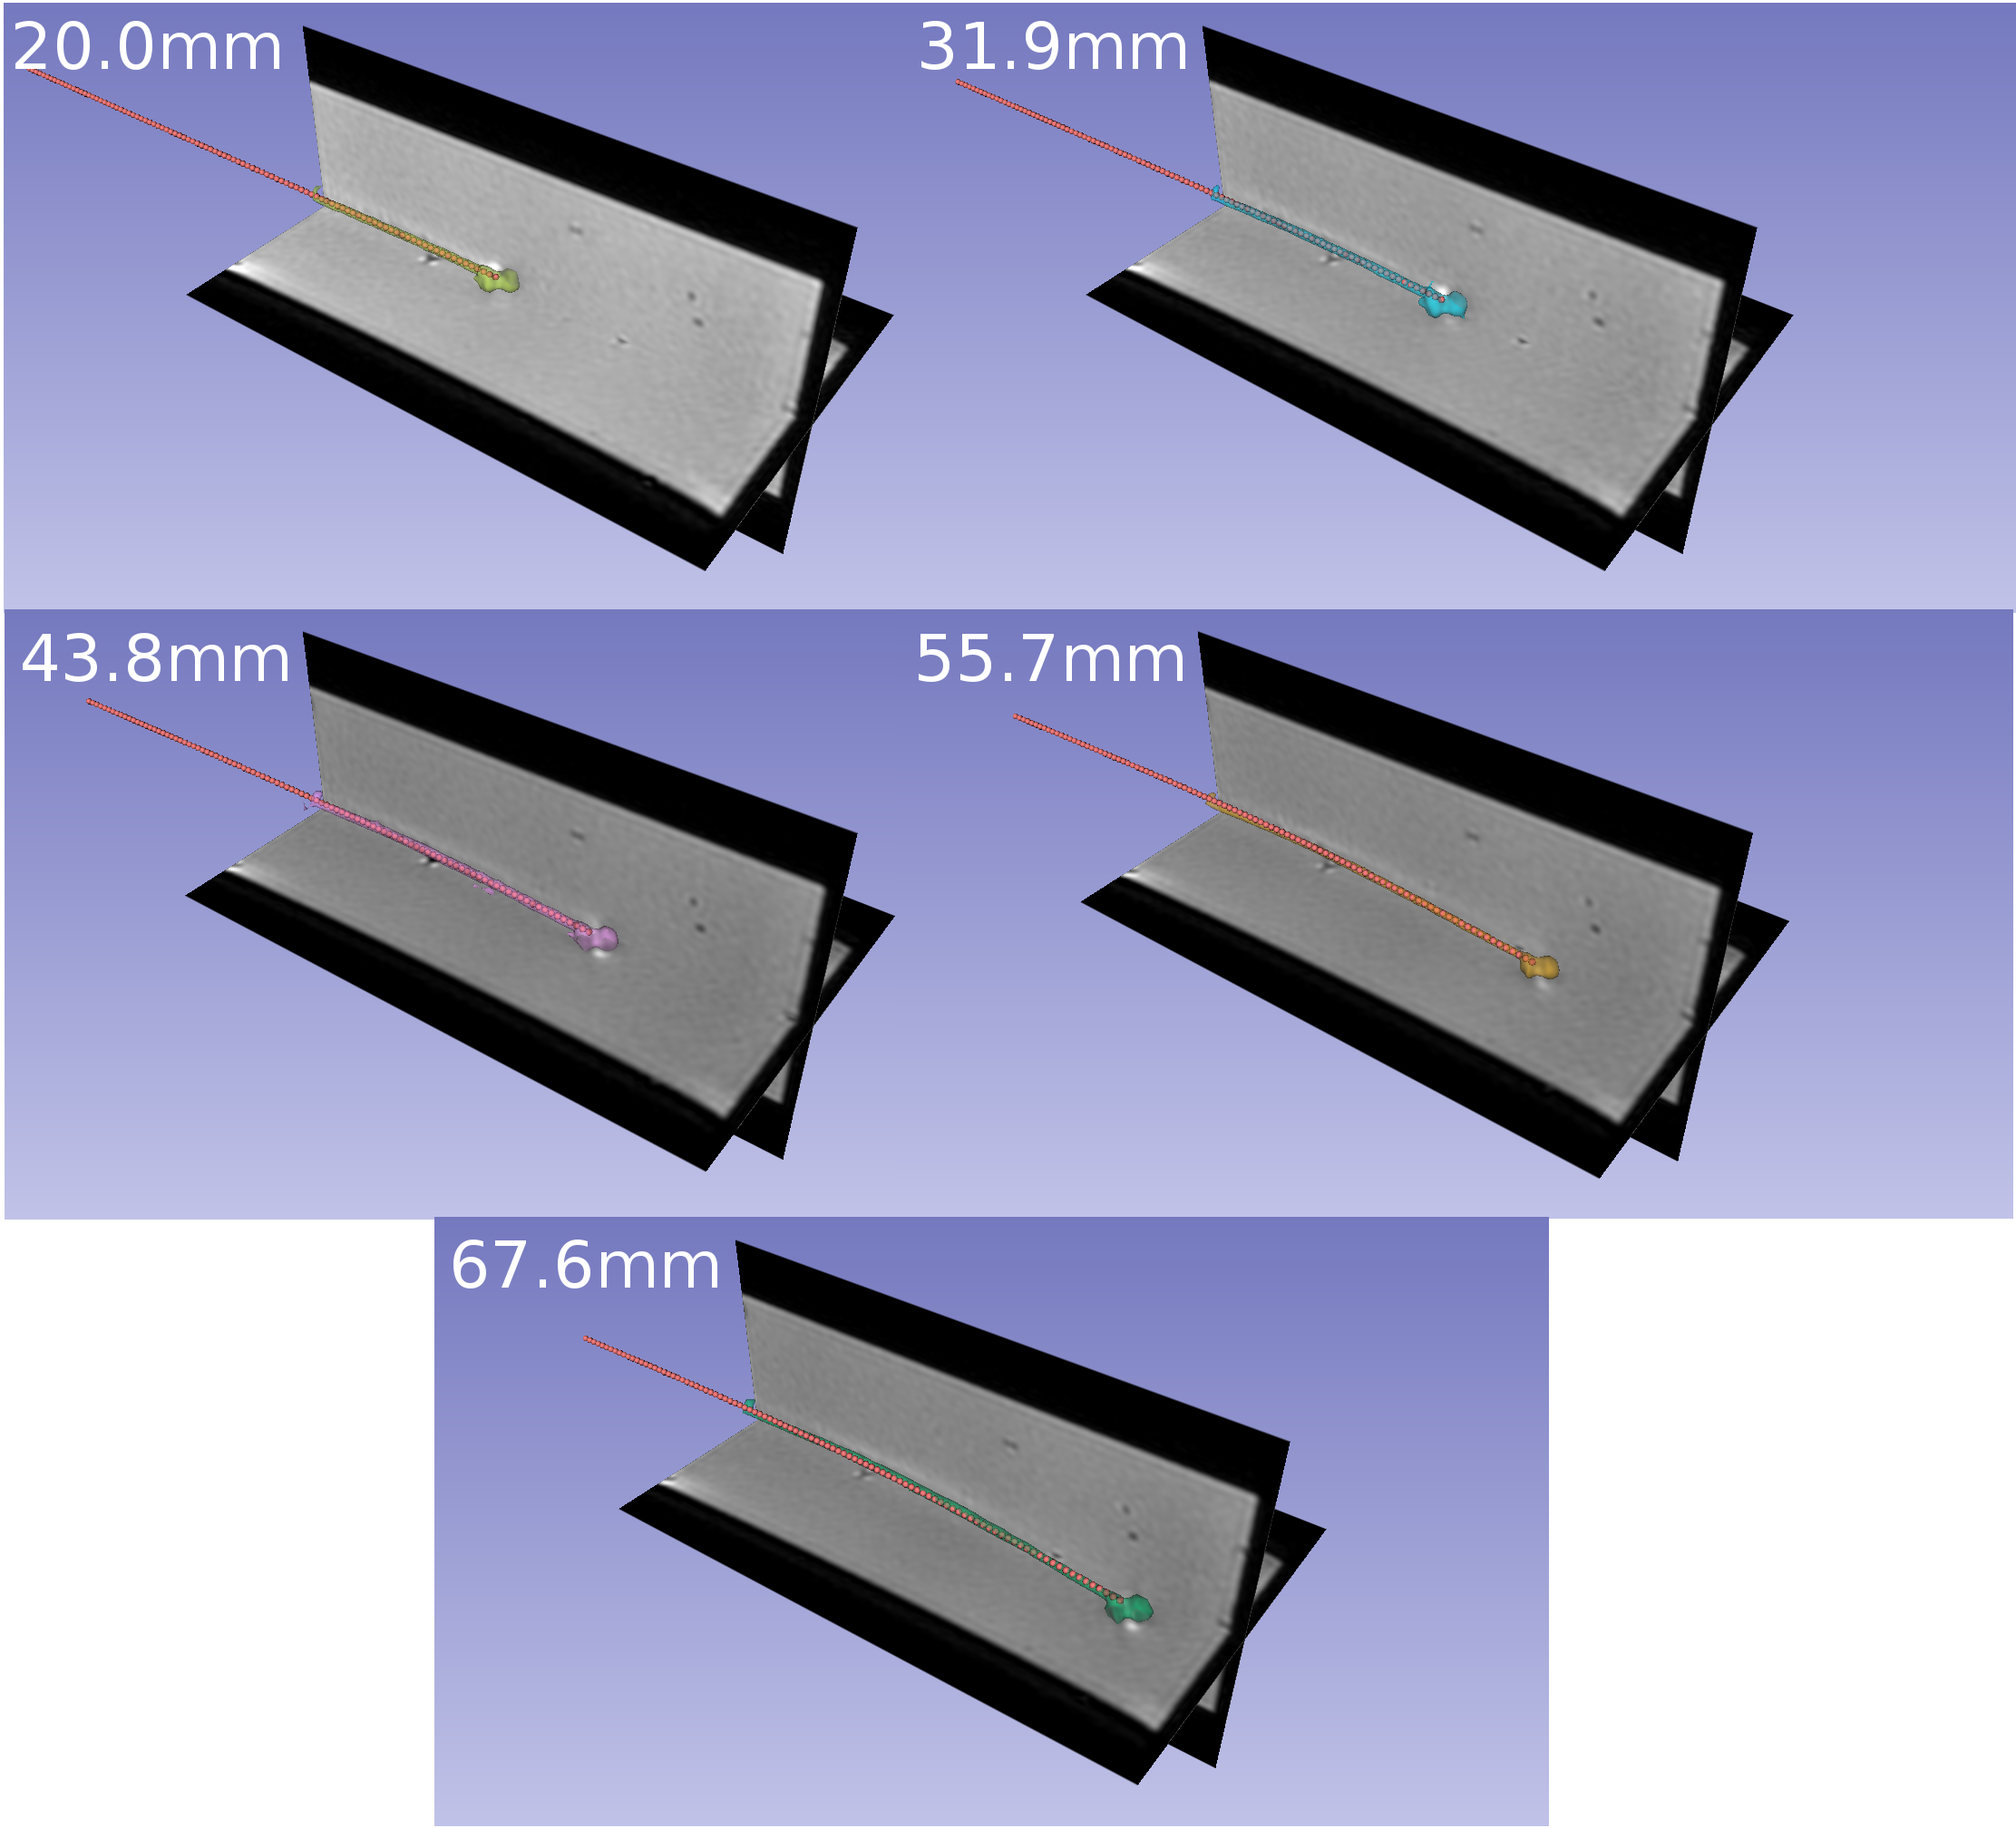
\includegraphics[width=1.0\textwidth]{Fig/chap5/insertions_labels.png}
\caption{Modeled curve points at each insertion step, with segmented artifact.}
\label{fig:curve_points}
\end{figure}

\begin{figure}[h]
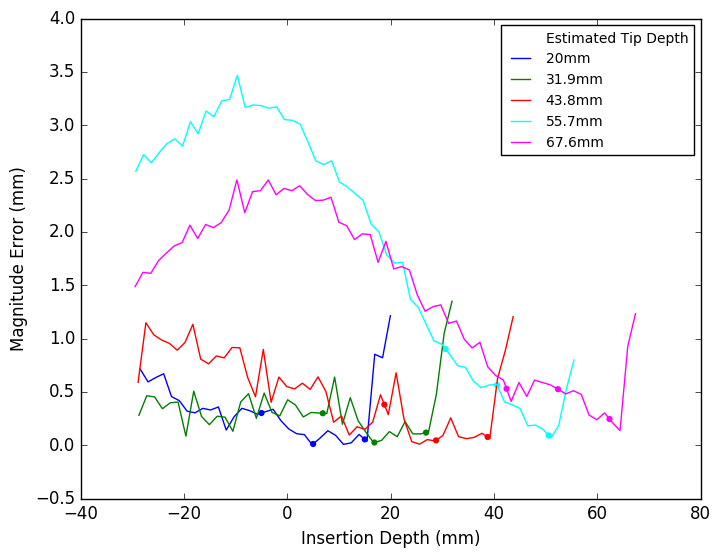
\includegraphics[width=1.0\textwidth]{Fig/chap5/error_curve_3_10.png}
\caption{Magnitude of error between the needle model and the artifact centroid with fixed spacing between slices. Markers indicate slice positions. $d=10mm$, $k=3$, $\delta=5mm$}
\label{fig:curve_errors_fixed_spacing}
\end{figure}

\begin{figure}[h]
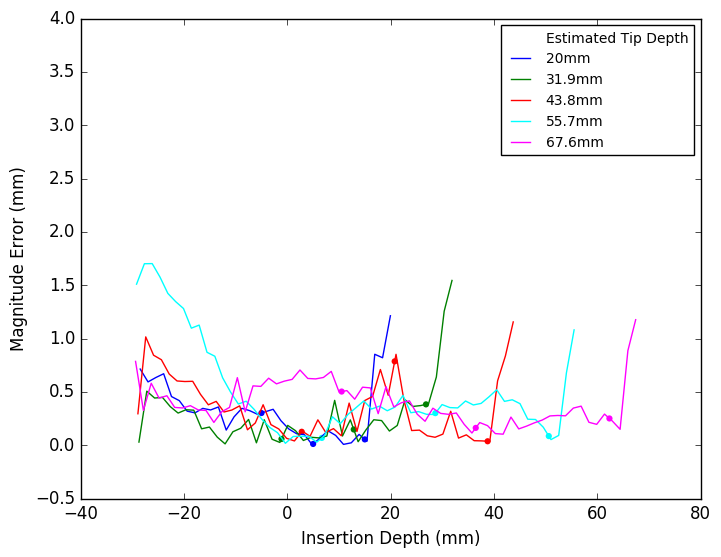
\includegraphics[width=1.0\textwidth]{Fig/chap5/error_curve_3_var.png}
\caption{Magnitude of error between the needle model and the artifact centroid, where the spacing between each slice increases with insertion depth. Markers indicate slice positions. $d=10mm + index_{step}*4mm$, $k=3$, $\delta=5mm$ }
\label{fig:curve_errors_variable_spacing}
\end{figure}



% %%%%%%%%%%%%%%%%%%%%% chapter.tex %%%%%%%%%%%%%%%%%%%%%%%%%%%%%%%%%
%
% sample chapter
%
% Use this file as a template for your own input.
%
%%%%%%%%%%%%%%%%%%%%%%%% Springer-Verlag %%%%%%%%%%%%%%%%%%%%%%%%%%

%\begin{savequote}[8cm]
%  ``Veni, vidi, vici.''
%  \qauthor{Julius Caesar}
%\end{savequote}


\chapter{Needle Localization in Stereo Images}
\label{sec:cameratracking} % Always give a unique label
% use \chaptermark{}
% to alter or adjust the chapter heading in the running head

Camera-based needle tracking is useful for the development of needle insertion systems.

Important to demonstrate compatibility with real-time insertion, and interoperability with the insertion robot.

Can test many more insertions than in MRI, due to shorter turnaround time, better availability, and less expensive operation.

\section{Vision Systems}
\subsection{Hardware}
The stereo tracking system used in this chapter was used previously in \cite{wartenberg_closed-loop_2017}. It uses two Logitech C920 USB webcams set to capture images at a resolution of 640px by 480px. The cameras are mounted in a highly-converging configuration, which each camera oriented normal to a face of the phantom.

- Add a picture of the camera setup

\subsection{Calibration and Registration}
- Add diagram of transforms between robot and cameras

	The stereo camera system was calibrated using the ROS camera calibration package, which bundles both intrinsic and extrinsic calibration into the same process. The origin of the stereo system is at the optical center of the side-mounted camera.
    
    A checkerboard marker mounted to a known position on the needle insertion robot allows the calculation of a transform relating the robot to the stereo system.
    
%     The highly-converging stereo arrangement presents challenges to accurate calibration. The camera fields of view intersect in a small volume, so there is a limited range of poses in which checkerboard corners are clearly visible in images from both cameras. Anecdotally, using two differently sized and shaped checkerboards in the same process produced better extrinsic calibration results in this highly-converging case than a single-checkerboard approach. The calibration patterns used were a 10x7 grid with 7mm squares and a 9x8 grid with 3.5mm squares. 
% 	Setting the stereo origin to be aligned with one camera is advantageous for testing and troubleshooting. The default outputs of the ROS stereo calibration node set the offset between the cameras in the Z-direction to be zero. The transform of the second camera in the frame of the first is an intermediate output of the node, so we can use it to construct projection matrices that place the stereo origin in a desirable orientation.
    


% 	ArUco markers are used throughout the registration process. The ArUco-augmented ChArUco checkerboard presents advantages over traditional checkerboard patterns since the uniquely-identified ArUco markers grant definitive directionality to the board in cases where the orientation of a normal board is ambiguous.
% 	Find pose of ChArUco calibration checkerboard in a removable plastic mount at a known position relative to the robot base. Save the transform between stereo frame and registration marker frame. Measured transforms are output in the frame of the registration marker. On the receiving end, the pose of registration marker relative to base frame is known, so measurements can be converted to be relative to the robot base frame.
    
% \subsection{Phantom Registration}
% 	Assume that phantom is a rectangular prism that can be represented as a box primitive. Create a custom ArUco board that fits one face of the phantom with markers along the top, bottom, and rear edges of the phantom face. Place the board origin at the center of the phantom. During registration find the pose of the board in images from the side camera. At the start of needle tracking initialize a triangular mesh to match the dimensions of the phantom and set its transform to match the one measured during registration.
% 	Other groups registering refracting volumes to camera systems have used different types of markers, such as colored spheres at the corners of a rectangular volume. The dependencies for the ArUco markers were already set up when the problem of phantom registration was approached, so it was convenient to use them.

\section{Needle Tracking Software}
- Add flowchart of software classes and data

% \subsection{Refraction Compensation}
% The index of refraction of PVC plastic mixed at a 7-to-3 ratio with softener agent was experimentally measured to be about 1.5.

% The dimensions and position of the phantom relative to the camera frame is defined by a user-specified box primitive represented by a triangular-faced mesh.

% Refraction compensation is required to correct for error in the observed positions of objects measured far from the interface between air and a refracting medium such as water, plastic, or glass, especially when the direction of observation meets the interface at an angle. \cite{Muller2014Refraction} presents a method for refraction compensation designed for estimating the poses of fish within an aquarium. The problem of observing a moving object in a transparent plastic phantom is similar in terms of the arrangement of the refracting body and moving objects relative to fixed cameras.

% A simulated ray is cast from the position of each camera to the measured position of the needle tip through the mesh. The location of the intersection with the phantom mesh and the normal direction of the intersected face are detected. The angle between the ray and the surface normal is calculated. The angle on the opposite side of the refractive interface is calculated via Snell's Law using the indices of refraction of the phantom material and the surrounding environment. The ray is rotated by the difference between the outside and inside angles about the point of intersection in the plane containing the ray and the surface normal. The closest point between the refracted rays from both stereo cameras is the actual position of the needle tip within the phantom.

\subsection{Forward Kinematics}
- Receive output of insertion robot forward kinematics via OpenIGTLink

- Data is the transform from stereo camera frame to needle tip assuming that the needle is rigid

- Use needle length to calculate transform from stereo camera frame to needle base


\subsection{Image Sampling}
Sequence of operations is designed to be very similar to imaging in MRI. 

Use transform between cameras and needle base and the previous model of the needle to find the position in the image just behind the needle tip.

-ample pixels in a column perpendicular to the direction of needle insertion at the point close to the tip and at N other points spaced along the needle shaft

\section{Experiments}
- Ground truth is sampling the entire length of the needle

- Compare sampling only a few points along the needle and fitting the various curve models

- Bending energy mechanical model

- Generic lower-degree polynomials

- Linear fit

\section{Results}
\begin{figure}[h]

\includegraphics[width=8cm]{Fig/placeholder.jpg}
\caption{Magnitude of in-plane error over insertion depth for each type of needle model.}
\label{fig:results_error}
\end{figure}

\begin{figure}[h]

\includegraphics[width=8cm]{Fig/placeholder.jpg}
\caption{Magnitude of in-plane error for the highly-curving needle case.}
\label{fig:pose_error}
\end{figure}

\begin{figure}[h]

\includegraphics[width=8cm]{Fig/placeholder.jpg}
\caption{Magnitude of needle tip pose orientation error for each type of needle model.}
\label{fig:pose_error}
\end{figure}

\begin{figure}[h]

\includegraphics[width=8cm]{Fig/placeholder.jpg}
\caption{Calculated needle tip trajectory for each type of needle model over the full length of insertion.}
\label{fig:pose_error}
\end{figure}

- Beam bending energy model gives a similar result to the least-squares model with fewer sampled points.

- Useful when sampling is expensive.

- Bending energy model also accommodates torturous needle trajectories due to parameterization of position in each axis.

    

    

    
% \section{Needle Tracking}
%     Noise and extraneous motion is filtered by thresholding the flow direction to within a range close to the expected needle insertion and retraction directions, and by thresholding the flow magnitude to a value above the observed maximum when no needle is present. 

% Dense optical flow processing time is reduced by only analyzing a limited subsection of each video frame. This rectangular subsection is centered at the last tip coordinate and clamped to the boundaries of the frame.

% Since this algorithm detects all motion in the camera field of view, the environment around the phantom must be controlled to eliminate motion other than the needle tip.

% \section{2D Validation}
% Compared manually-selected needle tip coordinates with those provided by DOF algorithm. [CITE New Paper]

% [INCLUDE PLOT]

% \section{3D Validation}
% Used OptiTrack to produce ground truth data for needle tip pose. [Cite New Paper]

% [INCLUDE PLOT]


\chapter{Conclusions and Future Extension}
\label{conclusions} % Always give a unique label


\section{Discussion}
- Resampling needle cross sections produces a better needle model than only tracking the tip, since the needle shaft deflects because of the elasticity of the phantom material.

- Linear regression is inadequate. Lowish-order polynomial regression works decently if there are many measurements and if the needle isn't subject to multiple bends.

- Minimum bending energy curve fitting works well with fewer data points than regression, but it can be slow if the initial estimates are not near to the final parameters, or if many curve segments are to be solved at the same time. There isn't any particular benefit to working with higher-degree polynomials, especially if the measured needle points are only associated with the end points of the curves.

- MBE for a single curve is less accurate than a piecewise curve, but the complexity of implementation and the time to solve is greatly reduced.

\section{Future Work}
- Need to implement communication with the MRI scanner to programmatically control scan planes, fields of view, protocols, etc. This was done previously as part of Nirav's PhD work but it was limited to a specific model of scannerl.

- Need better needle control algorithms to steer the needle along a trajectory, rather than just to a target point. 

- Demonstrate MRI simulation of needle artifacts

- Package and release stereo vision system and software

- Demonstrate MRI needle tracking using an actual MRI machine during a live insertion.

Volumetric imaging would present several benefits to 3D tracking, but the comparatively long scan times required (30 seconds according to \cite{BiopsyReview}) would limit its usefulness for real-time control in situations representative of clinical use. If the two-plane approach goes together easily, then I will pursue more advanced imaging methods.

It is expensive and time-consuming to test on actual MRI hardware. A needle insertion software simulation that returned MR-style imagery would be useful for early testing and development. This could probably be developed from a high-resolution 3D volumetric scan of a representative pelvic region.

The computer vision needle tracking software I developed in Spring 2017 is a useful tool for evaluating needle control methods, and I could continue developing it through 2018.


% \section{Summary of Work and Contributions}
% An overview of this work is presented below with a summary of contributions and lessons learned along the way.

% \begin{itemize}
% \item
% \textbf{Contribution 1}

% Contribution 1

% \item
% \textbf{Contribution 2}

% Contribution 2

% \item
% \textbf{Contribution 3}

% Contribution 3

% \end{itemize}

% \section{Impact and Future Work}
% The research presented in this dissertation addresses several major challenges.

% %\begin{itemize}
% \textbf{Impact}

% Here is the impact of my work.

% %\item 
% \textbf{Lessons Learned}

% Some lessons I've learned.

% %\item 
% \textbf{Future Work}

% Future work includes...

%\end{itemize}

%% REFERENCES
% if you use BIBTEX
\begin{spacing}{1}
\def\dsp{\def\baselinestretch{1.25}\large\normalsize}
\bibliographystyle{IEEEtran}
\bibliography{Zotero}
% \bibliography{Thesis_Needle_Guidance}

\end{spacing}
\end{document}
